\chapter{Detecting Refactoring in Version Histories}
\label{ChTse}

\noindent\textit{Identifying refactoring operations in source code changes is valuable to understand software evolution.
Therefore, several tools have been proposed to automatically detect refactorings applied in a system by comparing source code between revisions.
The availability of such infrastructure has enabled researchers to study refactoring practice in large scale, leading to important advances on refactoring knowledge.
However, although a plethora of programming languages are used in practice, the vast majority of existing studies are restricted to the Java language due to limitations of the underlying tools.
This fact poses an important threat to external validity.
Thus, to overcome such limitation, we propose RefDiff~2.0, a multi-language refactoring detection tool.
Our approach leverages techniques proposed in our previous work and introduces a novel refactoring detection algorithm that relies on the Code Structure Tree (CST), a simple yet powerful representation of the source code that abstracts away the specificities of particular programming languages.
Despite its language-agnostic design, our evaluation shows that RefDiff's precision (96\%) and recall (80\%) are on par with state-of-the-art refactoring detection approaches specialized in the Java language.
Our modular architecture also enables one to seamlessly extend RefDiff to support other languages via a plugin system.
As a proof of this, we implemented plugins to support two other popular programming languages: JavaScript and C.
Our evaluation in these languages reveals that precision and recall ranges from 88\% to 91\%.
With these results, we envision RefDiff as a viable alternative for breaking the single-language barrier in refactoring research and in practical applications of refactoring detection.
}

\section{Introduction}

%Refactoring is a well-known technique to improve the design of a system and enable its evolution~\cite{Fowler:1999}.
%In fact, existing studies~\cite{MurphyHill2012, tsantalis_empiricalstudy, Kim:2012:FSE, kim-tse-2014, fse2016-why-we-refactor} present strong evidences that refactoring is frequently applied by development teams, and it is an important aspect of their software maintenance workflow.


Knowing about the refactoring activity in software projects is a valuable information to help researchers understand software evolution.
For example, past studies have used such information to shed light on important aspects of refactoring practice, such as: how developers refactor~\citep{MurphyHill2012}, the usage of refactoring tools~\citep{negara2013, MurphyHill2012}, the motivations driving refactoring~\cite{Kim:2012:FSE, kim-tse-2014, fse2016-why-we-refactor}, the risks of refactoring~\citep{Kim:2012:FSE, kim-tse-2014, Kim:2011, weissgerber2006refactorings, bavota2012does}, and the impact of refactoring on code quality metrics~\citep{Kim:2012:FSE, kim-tse-2014}.
Moreover, it is often important to keep track of refactorings when performing source code evolution analysis because files, classes, or functions may have their histories split by the refactorings such as \emph{Move} or \emph{Rename}~\cite{icse2018}.

Additionally, knowing which refactoring operations were applied in the version history of a system may help in several practical tasks.
For example, in a study by \cite{Kim:2012:FSE}, many developers mentioned the difficulties they face when reviewing or integrating code changes after large refactoring operations, which moves or renames several code elements. Thus, developers feel discouraged to refactor their code. If a tool is able to identify such refactoring operations, it can possibly resolve merge conflicts automatically. 
Moreover, diff visualization tools can also benefit from such information, presenting refactored code elements side-by-side with their corresponding version before the change.
Another application for such information is adapting client code to a refactored version of an API it uses~\citep{henkel2005catchup, Xing:2008:JDevAn}. If we are able to detect the refactorings that were applied to an API, we can replay them on the client code automatically.

%Although there are approaches capable of detecting refactorings automatically, there are still some issues that hinder their application. Specifically, the precision and recall of such approaches still need improvements.
%In this paper, we try to fill this gap by proposing RefDiff, an automated approach that identifies refactorings performed in the version history of a system.
%RefDiff employs a combination of heuristics based on static analysis and code similarity to detect 13 well-known refactoring types.
%When compared to existing approaches, RefDiff leverages existing techniques and also introduces some novel ideas, such as the adaptation of the classical TF-IDF similarity measure from information retrieval to compare refactored code elements, and a new strategy to compare the similarity of fields by taking into account the similarity of the statements that reads from or writes to them.

Given the importance of studying refactoring activity, we proposed RefDiff in previous work~\citep{msr2017}. RefDiff is an automated approach that identifies refactorings operations performed in the version history of Java systems.
By that time, our main goal was to provide a reliable tool to mine refactoring activity in a fully automated fashion, with better precision and recall than existing approaches. Since then, other approaches have emerged, such as RMiner~\citep{tsantalis2018rminer}, which enhanced precision to even higher standards.
%the state-of-the-art has evolved to even higher standards of precision with RMiner~\cite{tsantalis2018rminer}.
Today, the availability of such tools enables large-scale and in-depth empirical studies on refactoring practice~\citep{fse2016-why-we-refactor, icse2018}.

Nevertheless, despite the advancements in the field of refactoring detection, existing tools are all centered in the Java language.
Thus, we are still not able to mine refactoring activity in a vast amount of software repositories written in other programming languages.
By restricting refactoring research to a single programming language, we may get a biased understanding of the reality.
Moreover, the practical applications of such tools are hindered by the lack of support of other popular programming languages.

For all these reasons, in this paper we propose a multi-language refactoring detection approach, named as RefDiff~2.0, which is a complete redesign of its first version that introduces an extensible architecture.
In RefDiff~2.0, the refactoring detection heuristics are fully implemented in a common core, and support for programming languages is provided by plug-in modules.
%that works with a language-independent model that abstracts abstracting away the 
As a way to validate this architecture, we implemented and evaluated extension modules for three mainstream programming languages with distinct characteristics: Java, JavaScript (a widely popular dynamic programming language, used mostly to build web applications) and C (a procedural programming language, used mostly to implement system software).

Additionally, we reworked the refactoring detection heuristics of RefDiff to significantly improve its precision when compared to our previous work.
Now, RefDiff achieves 96.4\% of precision and 80.4\% of recall when evaluated in the Java dataset proposed by \cite{tsantalis2018rminer}, against 79.3\% of precision and 80.2\% of recall in its prior version.
Moreover, RefDiff's precision is on par with RMiner, the current state-of-the-art in Java refactoring detection (96.4\% vs. 98.8\%).
This is a relevant achievement because our approach is not specialized in a single language.

In summary, we deliver the following contributions in this work:
\begin{itemize}
\item A major extension of our refactoring detection approach proposed in previous work~\citep{msr2017}, which includes a redesign of its core to work with a language-independent model and improved detection heuristics.
\item A publicly available implementation\footnote{RefDiff and all evaluation data are public available in GitHub:\\
\url{https://github.com/aserg-ufmg/RefDiff}}
of our approach, with out-of-the-box support for Java, C, and Javascript.
\item An evaluation of the precision and recall of RefDiff using a large scale dataset of refactorings performed in real-world Java open source projects, comparing it with RMiner, a state-of-the-art tool for detecting refactorings in Java. As a byproduct of this evaluation, we also extend the dataset with new refactoring instances discovered by our tool.
\item An evaluation of the precision and recall of RefDiff in real-world C and Javascript open source projects.
\end{itemize}

The remainder of this paper is structured as follows.
Section~\ref{SecBackground} describes related work, discussing existing refactoring detection approaches.
%with a special focus on RMiner, which is the one we compare with RefDiff.
Section~\ref{SecApproach} presents the proposed approach in details.
Section~\ref{sec:eval:java} describes the design and results of a large scale evaluation of RefDiff in Java projects.
Section~\ref{sec:eval:js:c} describes the design and results of an evaluation of RefDiff in C and JavaScript projects.
Last, Section~\ref{SecConclusion} presents final remarks and concludes the paper.






\section{Background}
\label{SecBackground}

Empirical studies on refactoring rely on means to identify refactoring activity. Thus, different techniques have been proposed and employed for this task.
For example, \cite{MurphyHill2012} collected refactoring usage data using a plug-in that monitors user actions in the Eclipse IDE, including calls to refactoring commands.
%Negara~et~al.~\cite{negara2013} also used the strategy of instrumenting the IDE to infer refactorings from fine-grained code edits.
\cite{negara2013} describe a tool, called CodingTracker, to infer refactorings from fine-grained code edits. They use this tool to study refactorings performed by 23 developers working in their IDEs during a total of 1,520 hours. The tool achieved a precision of 99.3\% when evaluated with the automated Eclipse refactorings performed by the study participants.
On a sample of both manual and automated refactorings, CodingTracker achieved a precision of 93\% and a recall of 100\%.
However, CodingTracker requires the installation of a refactoring inference plugin in IDEs.

Other studies use metadata from version control systems to identify refactoring changes. For example, \cite{ratzinger2008relation} search for a predefined set of terms in commit messages to classify them as refactoring changes. In specific scenarios, a branch may be created exclusively to refactor the code, as reported by \cite{kim-tse-2014}.
Another strategy is employed by \cite{soares2010making}. They propose an approach that identifies behavior-preserving changes by automatically generating and running test-cases. While their approach is intended to guarantee the correct behavior of a system after refactoring, it may also be employed to classify commits as behavior-preserving.
Moreover, many existing approaches are based on static analysis.
This is the case of the approach proposed by \cite{demeyer2000finding}, which finds refactored elements by observing changes in code metrics.

Static analysis is also frequently used to find differences in the source code by comparing two revisions~\citep{dig2006automated, weissgerber2006identifying, tsantalis_empiricalstudy,prete2010template,Kim:2010:RefFinder,msr2017,tsantalis2018rminer}.
Approaches based on comparing source code differences have the advantage of beeing able to identify refactoring operations applied in version histories.
As RefDiff is one of these approaches, it can be directly compared with others within this category. In the next sections, we discuss RefDiff~1.0 and three other approaches.

\subsection{RefDiff~1.0}

The original version of RefDiff~\citep{msr2017}, which we will denote as RefDiff~1.0 throughout this chapter, employs a combination of heuristics based on static analysis and code similarity to detect 13 well-known refactoring types.
One of its distinguishing characteristic is the use of the classical TF-IDF similarity measure from information retrieval to compute code similarity.
In our previous work, we evaluated RefDiff~1.0 using an oracle of 448 refactoring operations, distributed across seven Java projects.
We built this oracle by deliberately applying refactorings in software repositories in a controlled manner.
Although this strategy poses the risk of creating an artificial dataset, this way we assured this oracle was complete and could be used to compute both precision and recall.
We compared our tool with three existing approaches, namely Refactoring Miner~\citep{tsantalis_empiricalstudy}, Refactoring Crawler~\citep{dig2006automated}, and Ref-Finder~\citep{Kim:2010:RefFinder}.
Our approach achieved precision of 100\% and recall of 88\%, surpassing the three tools subjected to the comparison.


\subsection{Refactoring Miner/RMiner}

Refactoring Miner is an approach originally introduced by \cite{tsantalis_empiricalstudy}, capable of identifying 14 high-level refactoring types: \emph{Rename Package/Class/Method}, \emph{Move Class/Method/Field}, \emph{Pull Up Method/Field}, \emph{Push Down Method/Field}, \emph{Extract Method}, \emph{Inline Method}, and \emph{Extract Superclass/Interface}.
In its original version, Refactoring Miner employs a lightweight algorithm, similar to the UMLDiff proposed by \cite{Xing:2005}, for differencing object-oriented models, inferring the set of classes, methods, and fields added, deleted or moved between two code revisions. 
Refactoring Miner was employed and evaluated in empirical studies on refactoring along its evolution.
In the first study, using the version histories of JUnit, HTTPCore, and HTTPClient, \cite{tsantalis_empiricalstudy} reported 8 false positives for the \emph{Extract Method} refactoring (96.4\% precision) and 4 false positives for the \emph{Rename Class} refactoring (97.6\% precision). No false positives were reported for the remaining refactorings.
In a second study that mined refactorings in 285 GitHub hosted Java repositories~\citep{fse2016-why-we-refactor}, we found found 1,030 false positives out of 2,441 refactorings (63\% precision). However, we also evaluated Refactoring Miner using as a benchmark the dataset reported by \cite{Chaparro:2014}, in which it achieved 93\% precision and 98\% recall.

In a recent study, \cite{tsantalis2018rminer} proposed a major evolution of its tool, now named as RMiner.
In its current version, RMiner relies on an AST-based statement matching algorithm and a set of detection rules that cover 15 representative refactoring types. 
Its statement matching algorithm employes two techniques to be resilient to code restructuring during refactoring: abstraction, which deals with changes in statements' AST type due to refactorings, and argumentization, which deals with changes in sub-expressions within statements due to parameterization.
To evaluate RMiner, the authors created a dataset with 3,188 real refactorings instances from 185 open-source projects. Using this oracle, the authors found that RMiner has a precision of 98\% and recall of 87\%, which was the best result so far, surpassing RefDiff 1.0, the previous state-of-the-art, which achieved precision of 75.7\% and recall of 85.8\% in this dataset.


%that was later extend by Silva~et~al.~\cite{fse2016-why-we-refactor} to mine refactorings in large scale in git repositories. This tool is capable of identifying 14 high-level refactoring types: \emph{Rename Package/Class/Method}, \emph{Move Class/Method/Field}, \emph{Pull Up Method/Field}, \emph{Push Down Method/Field}, \emph{Extract Method}, \emph{Inline Method}, and \emph{Extract Superclass/Interface}.

%Refactoring Miner runs a lightweight algorithm, similar to the UMLDiff proposed by Xing and Stroulia~\cite{Xing:2005}, for differencing object-oriented models, inferring the set of classes, methods, and fields added, deleted or moved between two code revisions. 
%First, the algorithm matches code entities in a top-down order (starting from the classes and going to the methods and fields) looking for exact matches on their names and signatures (in the case of methods).
%Next, the removed/added elements between the two models are matched based only on the equality of their names in order to find changes in the signatures of fields and methods.
%Third, the removed/added classes are matched based on the similarity of their members at signature level.
%Finally, a set of rules enforcing structural constraints is applied to identify specific types of refactorings.



\subsection{Refactoring Crawler}

Refactoring Crawler, proposed by \cite{dig2006automated}, is an approach capable of finding seven high-level refactoring types: \emph{Rename Package/Class/Method}, \emph{Pull Up Method}, \emph{Push Down Method}, \emph{Move Method}, and \emph{Change Method Signature}.
It uses a combination of syntactic analysis to detect refactoring candidates and a reference graph analysis to refine the results.

First, Refactoring Crawler analyzes the abstract syntax tree of a program and produces a tree, in which each node represents a source code entity (package, class, method, or field).
Then, it employs a technique known as \emph{shingles encoding} to find 
similar pairs of entities, which are candidates for refactorings.
Shingles are representations for strings with the following property: if a string changes slightly, then its shingles also change slightly.
In a second phase, Refactoring Crawler applies specific strategies for detecting each refactoring type, and computes a more costly metric that determines the similarity of references between code entities in two versions of the system. For example, two methods are similar if the sets of methods that call them are similar, and the sets of methods they call are also similar.
The strategies to detect refactorings are repeated in a loop until no new refactorings are found. Therefore, the detection of a refactoring, such as a rename, may change the reference graph and enable the detection of new refactorings.

The authors evaluated Refactoring Crawler comparing pairs of releases of three open-source software components: Eclipse UI, Struts, and JHotDraw. Such components were chosen because they provided detailed release notes describing API changes. The authors relied on such information and on manual inspection to build an oracle
%of known refactorings in those releases
containing 131 refactorings.
The reported results are: Eclipse UI (90\% precision and 86\% recall), Struts (100\% precision and 86\% recall), and JHotDraw (100\% precision and 100\% recall).
However, in our previous study~\citep{msr2017}, Refactoring Crawler achieved only 41.9\% of precision and 35.6\% of recall.

\subsection{Ref-Finder}

Ref-Finder, proposed by \cite{prete2010template,Kim:2010:RefFinder}, is an approach based on logic programming capable of identifying 63 refactoring types from the Fowler's catalog~\citep{Fowler:1999}.
The authors express each refactoring type by defining structural constraints, before and after applying a refactoring to a program, in terms of template logic rules.

First, Ref-Finder traverses the abstract syntax tree of a program and extracts facts about code elements, structural dependencies, and the content of code elements, to represent the program in terms of a database of logic facts. Then, it uses a logic programming engine to infer concrete refactoring instances, by creating a logic query based on the constraints defined for each refactoring type.
The definition of refactoring types also consider ordering dependencies among them. This way, lower-level refactorings may be queried to identify higher-level, composite refactorings.
The detection of some types of refactoring requires a special logic predicate that indicates that the similarity between two methods is above a threshold. For this purpose, the authors implemented a block-level clone detection technique, which removes any beginning and trailing parenthesis, escape characters, white spaces, and return keywords and computes word-level similarity between the two texts using the longest common sub-sequence algorithm.

The authors evaluated Ref-Finder in two case studies.
In the first one, they used code examples from the Fowler's catalog to create instances of the 63 refactoring types. The authors reported 93.7\% recall and 97.0\% precision for this first study.
In the second study, the authors used three open-source projects: Carol, jEdit, and Columba. In this case, Ref-Finder was executed in randomly selected pairs of versions. From the 774 refactoring instances found, the authors manually inspected a sample of 344 instances and found that 254 were correct (73.8\% precision).
However, in a study by \cite{Soares:2013} using a set of randomly select revisions of JHotDraw and Apache Common Collections containing 81 refactoring instances in total, Ref-Finder achieved 35\% of precision and 24\% of recall.
Moreover, in our previous study~\citep{msr2017}, it also achieved 26.4\% of precision and 64.2\% of recall.

It is worth noting that Ref-Finder and Refactoring Crawler require a full build of the program under analysis.
Therefore, their usage is not recommended when mining refactorings from version histories in the large.
In this case, it might be a challenge to build each release, due to missing external dependencies, for example.
For that reason, our evaluation (Section~\ref{sec:eval:java}) focus on comparing RefDiff with RMiner.




\section{Proposed Approach}
\label{SecApproach}

Our approach consists of two phases: Source Code Analysis and Relationship Analysis.
In the first phase, Source Code Analysis, we take as input two revisions of a system, $v_1$ and $v_2$, and build two models that represent their source code.
Both models have the form of a tree, in which each node corresponds to a code element (classes, functions, etc.).
In the second phase, Relationship Analysis, we compute a set $R$, which contains triples of the form $(n_1, n_2, t)$, where $n_1$ is a code element from revision $v_1$, $n_2$ is a code element from revision $v_2$ and $t$ is a relationship type.
Such relationships may denote a high-level refactoring operation (move, rename, extract, etc.) or an exact correspondence between the code elements.
For example, consider the diff between two revisions of a system depicted in Figure~\ref{FigDiff1}.
Among other changes, the class \codeinl{Calculator}, declared in revision~1, is renamed to \codeinl{FpCalculator} in revision~2. This corresponds to a relationship of the type \emph{Rename} between them.
In the next sections, we describe in details each phase of our approach.

\begin{figure*}[htb]
\centering
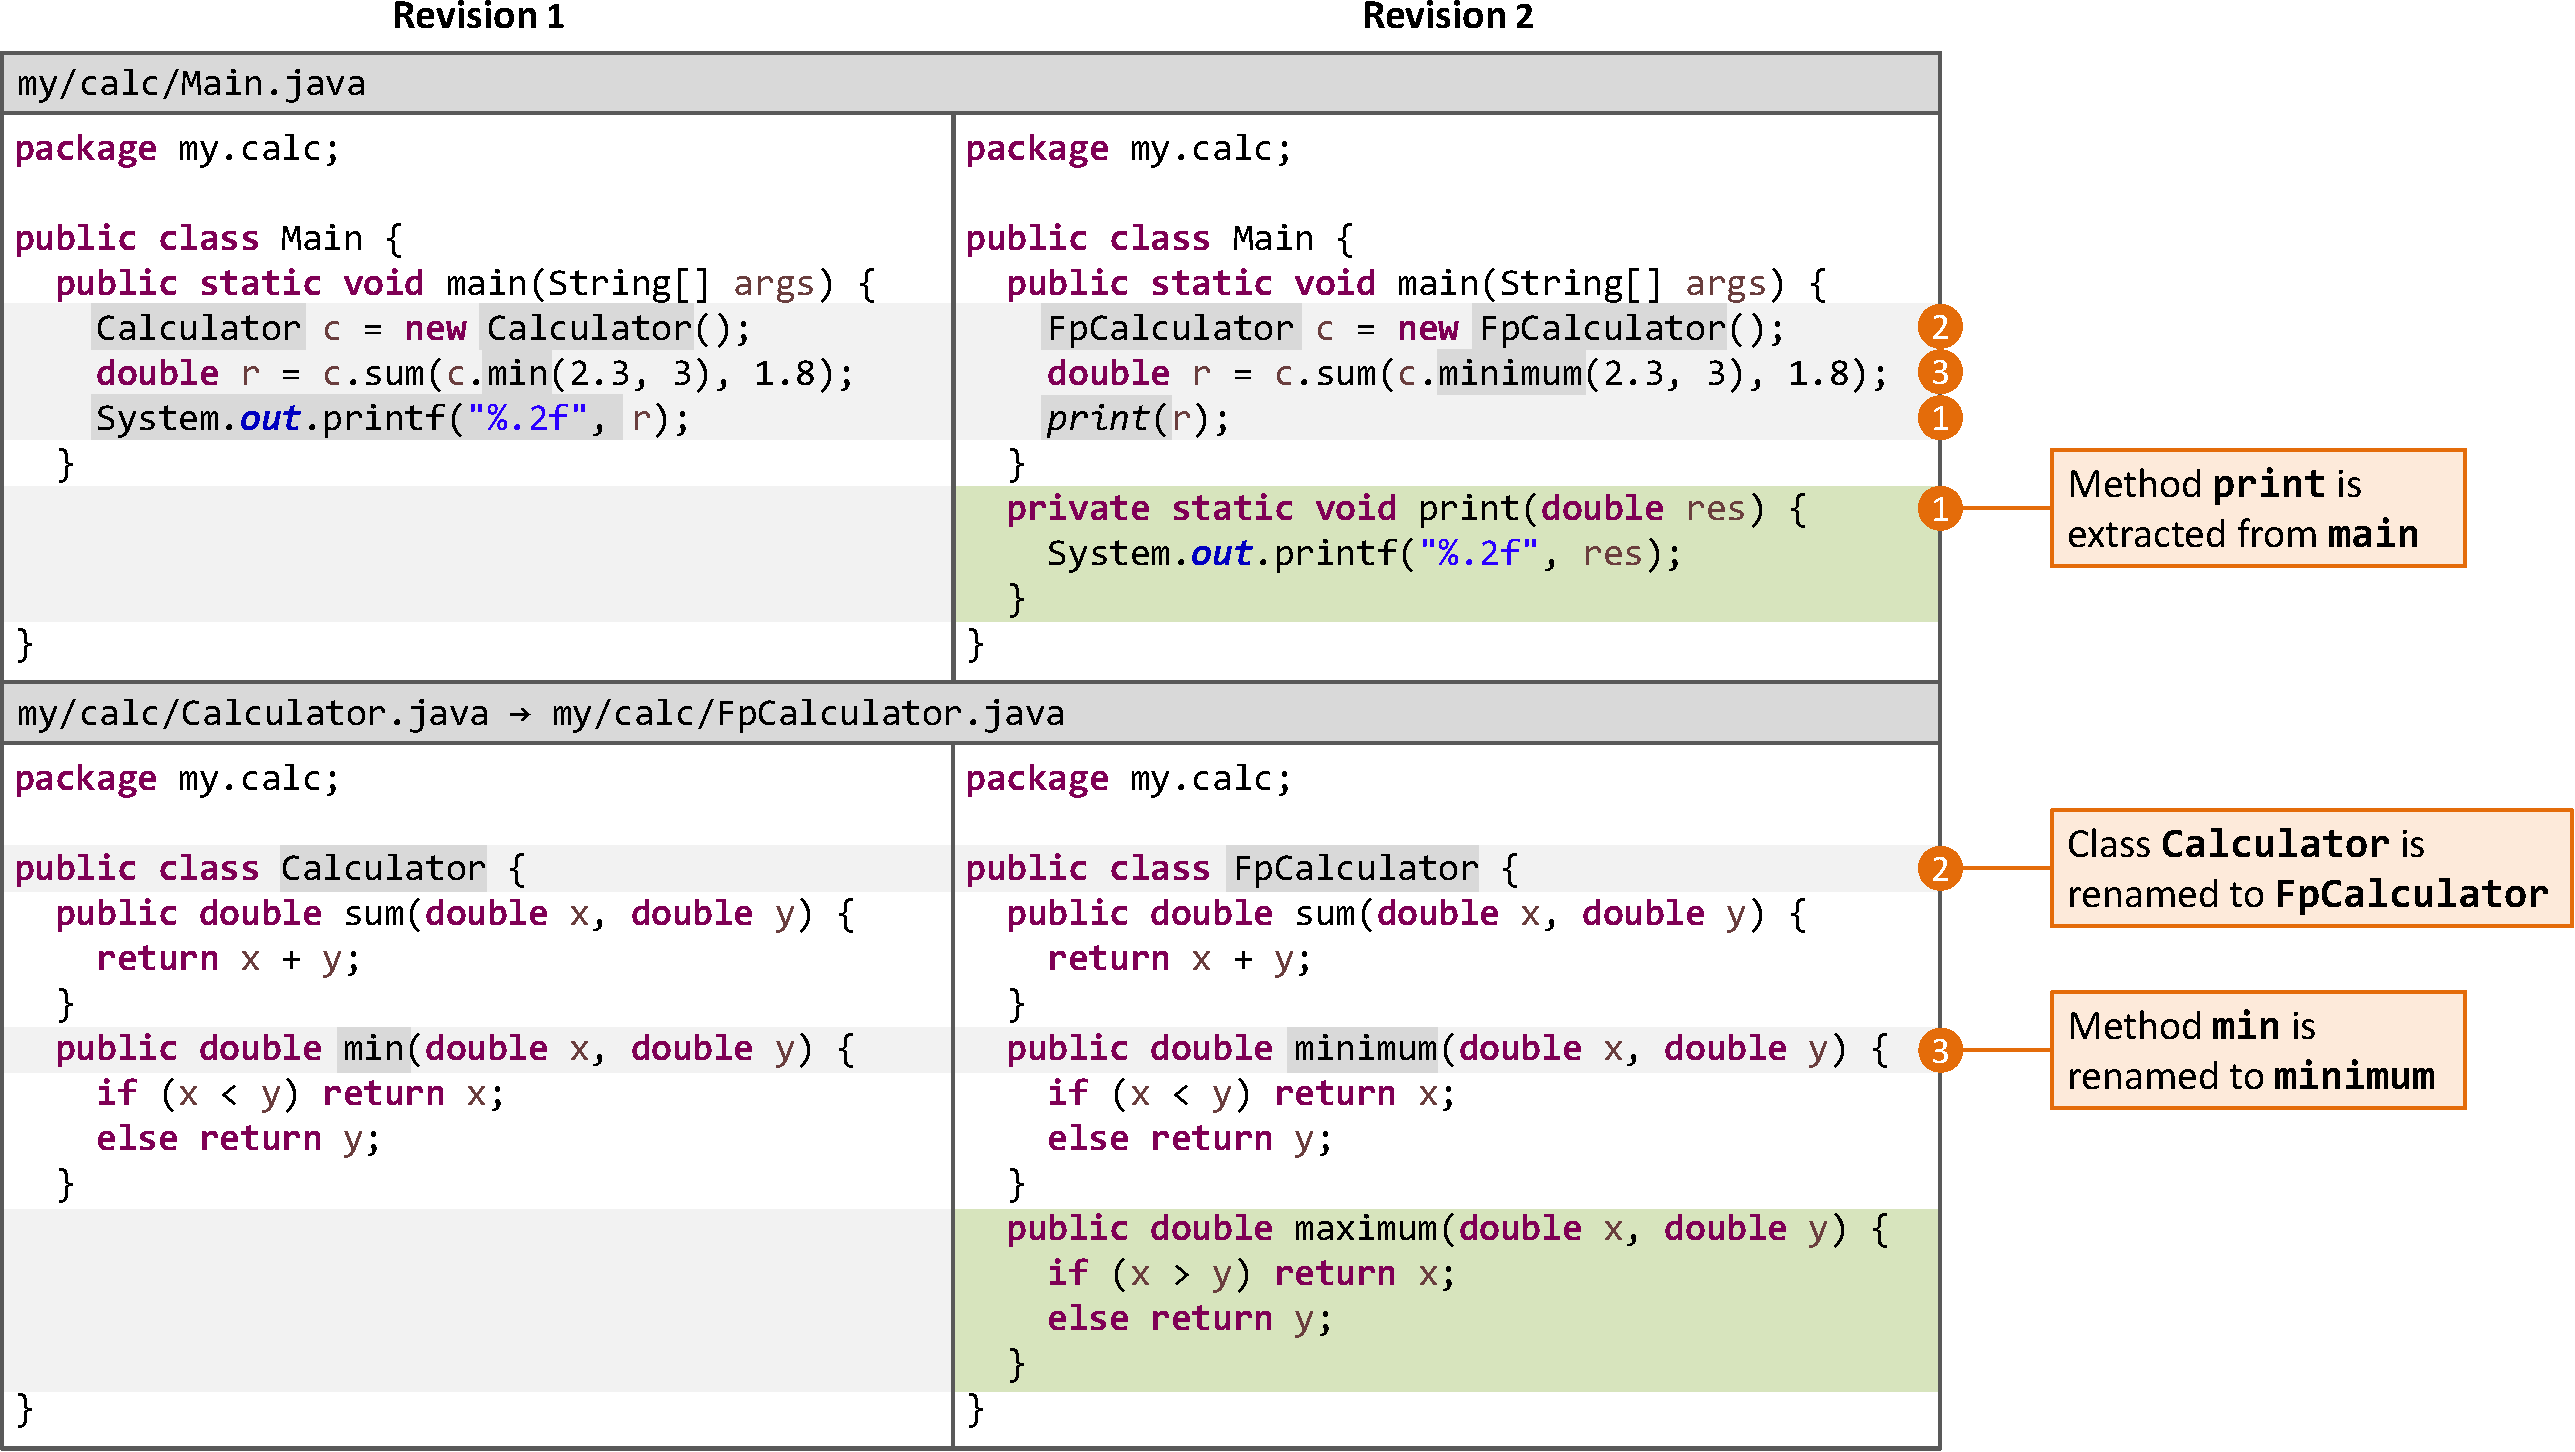
\includegraphics[width=1.0\textwidth]{img/diff1.pdf}
\caption{Illustrative diff between two revisions of a system annotated with refactoring operations}
\label{FigDiff1}
\end{figure*}


\subsection{Phase 1: Source Code Analysis}

The goal of this phase is to compute a language-independent model that represents the source code of the system, which we denote from now on as \emph{Code Structure Tree} (CST). The CST is a tree-like structure that resembles an \emph{Abstract Syntax Tree} (AST). However, in this representation we are only interested in coarse-grained code elements (e.g., classes and functions) that encompass a code region and may be referred by an identifier in other parts of the system.

To construct the CST, we need to parse the source code, generate the AST for the target programming language, and extract the necessary information.
Thus, the decision of which types of AST nodes become CST nodes depends on the programming language.
For example, in Java we represent classes, enums, interfaces, and methods as CST nodes.
In contrast, local variables are not represented.
Nevertheless, it is important to note that the granularity of the CST nodes determines the granularity of the relationships we are able to find, e.g., we can only find relationships between methods if we represent methods in the CST.
Table~\ref{TabCstNodes} lists the types of AST nodes that are represented in the CST for each programming language supported by the current implementation of our approach.

\begin{table}[htbp]
\renewcommand{\arraystretch}{1.2}
\caption{AST nodes that are represented in CSTs}
\label{TabCstNodes}
\centering
\begin{tabular}{@{}ll@{}}
\toprule
Language & Node types \\
\midrule
Java & class, enum, interface, and method \\
C & file and function \\
JavaScript & file, class, and function \\
\bottomrule
\end{tabular}
\end{table}

\begin{figure}[htb]
\centering
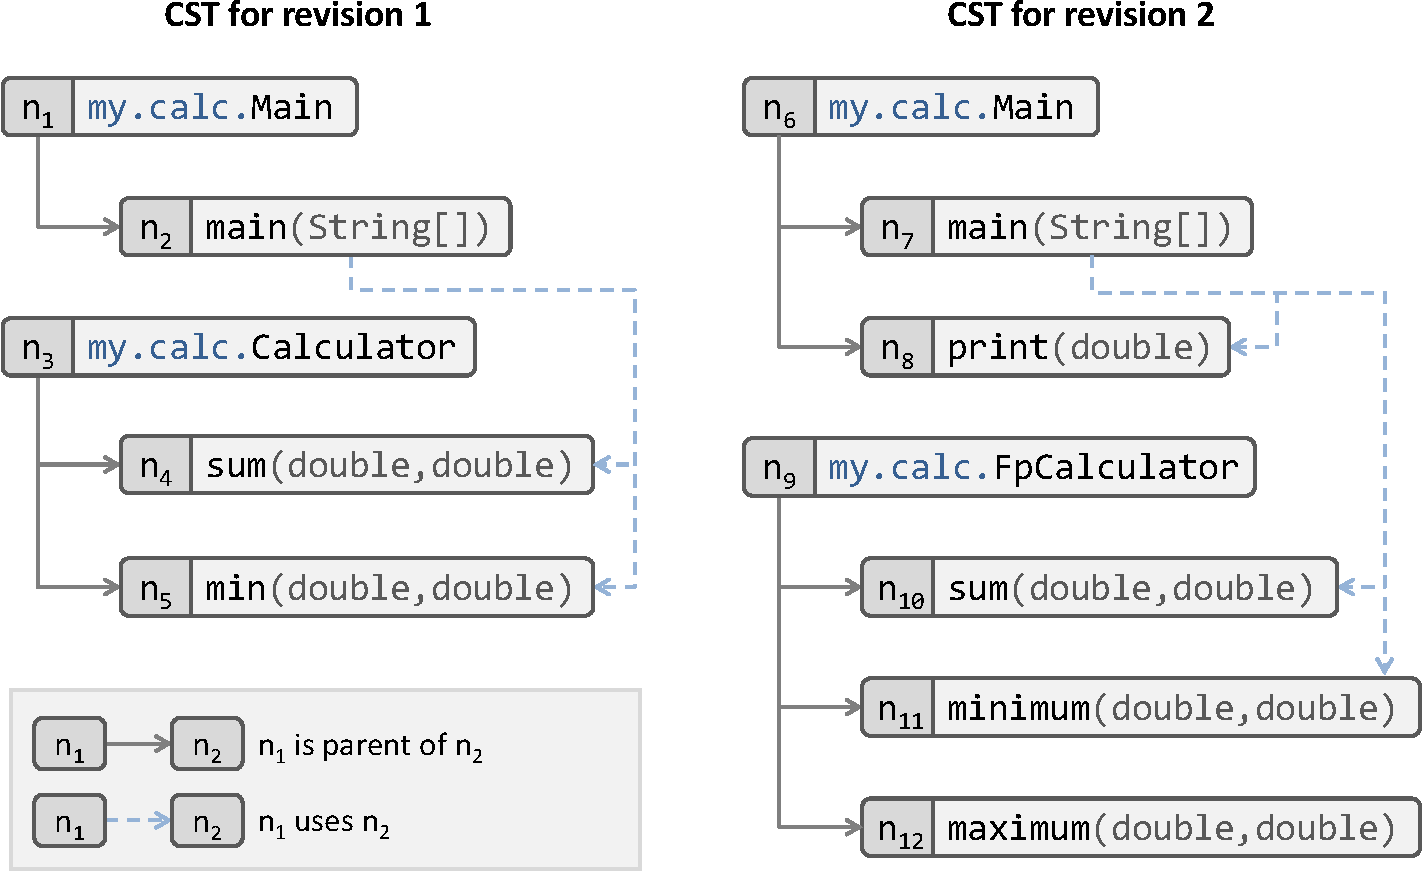
\includegraphics[width=0.75\linewidth]{img/cstDiff1.pdf}
\caption{CST of both revisions of the example system from Figure~\ref{FigDiff1}}
\label{FigJavaToCst}
\end{figure}

Figure~\ref{FigJavaToCst} exemplifies the transformation of the example system from Figure~\ref{FigDiff1} into a corresponding CST.
In revision~1, the class \codeinl{Main} is declared with a single method \codeinl{main} and the class \codeinl{Calculator} contains two methods: \codeinl{sum} and \codeinl{min}.
Note that these classes and methods become nodes in the CST for revision~1, preserving the same nesting structure of the source code. Analogously, the figure also depicts the CST for revision 2, which contains seven nodes in total (two classes and five methods).

Besides the representation of the code elements, the CST also embeds a simplified call graph and  a type hierarchy graph of the nodes within the CST, that is, there are edges to represent whether a certain node $n_1$ calls $n_2$, or whether $n_1$ is a subtype of $n_2$. The first information is necessary to find \emph{Extract} and \emph{Inline} relationships between code elements, while the second is used to find inheritance-related relationships, such as \emph{Pull Up} and \emph{Push Down}.

Moreover, along with each node of the CST, we store the following information:
\begin{description}
    \item[Identifier] \hfill \\
    An identifier of the code element in its declared scope. 
    The identifier is usually the name of the code element, but it may also contain additional information to avoid ambiguities.
    For example, the identifier of the class \codeinl{Calculator} from Figure~\ref{FigJavaToCst} is simply its name, but the identifier of the method \codeinl{sum} is \codeinl{sum(double,double)},  because there could be an overloaded method with a different signature.
    
    \item[Namespace] \hfill \\
    An optional prefix that, along with the identifier, globally identifies the code element. 
    This information only applies to top-level nodes and corresponds to the package or folder that the element is contained. For example, the namespace of the class \codeinl{Calculator} from Figure~\ref{FigJavaToCst} is \codeinl{my.calc.}.
    
    \item[Node type] \hfill \\
    A string that identifies the node type in the target language (class, function, method, etc.).
    
    \item[Parameters list]  \hfill \\
    An optional list of the name of the parameters, in the case the node corresponds to a method or function.
    
    \item[Tokenized source code]  \hfill \\
    The source code of the element in the form of a list of tokens.
    Here, we include all tokens in the code region that encompasses the complete declaration of the code element, including its name/signature.
    This information is necessary to compute the similarity between code elements, as explained in Section~\ref{SecCodeSim}.
    
    
    \item[Tokenized source code of the body]  \hfill \\
    The source code of the body of the code element in the form of a list of tokens.
    Here we include only the tokens within the body of the code element, but not its name/signature.
    This information is also necessary to compute the similarity between code elements in the special cases of \textit{Extract} and \textit{Inline} relationships, as explained in Section~\ref{SecSimX}.
    It is worth noting that this information is optional, as not every node has a body (e.g., abstract methods).
    
\end{description}

It is worth noting that we generate the CST only for source files that have been added, removed, or modified between revisions. 
Such information can be efficiently obtained from version control systems, without the need to analyze the content of all files within the repository.
This way, we avoid a costly operation that might compromise the scalability of our approach, as large repositories contain thousands of source files, but only a small fraction of them change between revisions.

Although the construction of the CST is a language-specific process, from this point on, the approach is language-independent and relies only on information encoded in CSTs.
This way, one is able to extend our approach to work with different programming languages only by implementing the \emph{Source Code Analysis} module.
To demonstrate this capability, we provide implementations for three programming languages: Java, C, and JavaScript.


\subsection{Phase 2: Relationship Analysis}

This phase takes as input the CST's of revisions $v_1$ and $v_2$ and outputs the set of relationships $R$. Let $N_1$ and $N_2$ be the sets of code elements from the CST's of $v_1$ and $v_2$ respectively. Each relationship $r \in R$ is a triple $(n_1, n_2, t)$, where $n_1 \in N_1$, $n_2 \in N_2$, and $t$ is a relationship type. The types of relationships are listed in the first column of Table~\ref{TabRelationshipTypes}, and can be subdivided into two groups:
\begin{itemize}
\item \textbf{Matching relationships}, which indicate that the node $n_1$ corresponds to $n_2$ in the subsequent revision.
The possible matching relationships are \textit{Same}, \textit{Convert Type}, \textit{Pull Up}, \textit{Push Down}, \textit{Change Signature}, \textit{Move}, \textit{Rename}, and \textit{Move and Rename}.
We say that a node $n_1$ matches with $n_2$ if exists a relationship $(n_1, n_2, t) \in R$ such that $t$ is a matching relationship.

\item \textbf{Non-matching relationships}, which indicate that either node $n_1$ is decomposed to create $n_2$, or node $n_1$ is incorporated into $n_2$.
There are four non-matching relationships: \textit{Extract Supertype}, \textit{Extract}, \textit{Extract and Move}, and \textit{Inline}.
\end{itemize}


\subsubsection{General algorithm to find relationships}

Our approach employs the algorithm described in Figure~\ref{AlgoGeneral} to find the relationships (i.e., to compute the set $R$).
The procedure \textsc{FindRelationships} has two parameters, $t_1$ and $t_2$, which are the root nodes of the CST's of both revisions.
Initially, we define $R \gets \emptyset$ as the set of relationships found so far (line~2).
Additionally, we also define $M \gets \emptyset$ as the set of pairs of matching nodes found so far (line~3).
Then, we execute four subroutines:

\begin{figure}[htbp]
%\small
\fontsize{9.5}{10.5}\selectfont
\begin{algorithmic}[1]
\Procedure{FindRelationships}{$t_1,t_2$}
\State $R \gets \emptyset$
\State $M \gets \emptyset$
\State $\textsc{findMatchingsById}(t_1,t_2)$
\State $\textsc{findMatchingsBySim}$
\State $\textsc{findMatchingsByChildr}$
\State $\textsc{resolveMatchings}$
\State $\textsc{findNonMatchingRel}$
\State \Return $R$
\\
\Procedure{findMatchingsById}{$p_1,p_2$}
\ForEach{$(n_1, n_2) \in \rdchildren(p_1) \times \rdchildren(p_2)$}
  \If {$\rdsig(n_1) = \rdsig(n_2) \land \rdns(n_1) = \rdns(n_2)$}
    \State $\textsc{addMatch}(n_1, n_2)$
  \EndIf
\EndFor
\EndProcedure
\\
\Procedure{findMatchingsBySim}{}
\ForEach{$(n_1, n_2) \in \rdsortbysim(N^- \times N^+)$}
  \If {$\mathit{findMatchRel}(n_1, n_2) \neq \emptyset$}
    \State $\textsc{addMatch}(n_1, n_2)$
  \EndIf  
\EndFor
\EndProcedure
\\
\Procedure{findMatchingsByChildr}{}
\ForEach{$(n_1, n_2) \in \rdsortbysim(N^- \times N^+)$}
  \If {$\mathit{matchingChildr}(n_1, n_2) > 1\,\land \rdnsim(n_1, n_2) > 0.5$}
    \State $\textsc{addMatch}(n_1, n_2)$
  \EndIf
\EndFor
\EndProcedure
\\
\Procedure{resolveMatchings}{}
\ForEach{$(n_1, n_2) \in M$}
  \State $R \gets R \cup \mathit{findMatchRel}(n_1, n_2)$
\EndFor
\EndProcedure
\\
\Procedure{findNonMatchingRel}{}
\ForEach{$(n_1, n_2) \in M_1 \times N^+$}
  \State $R \gets R \cup \mathit{findExtractSupertype}(n_1, n_2)$
  \State $R \gets R \cup \mathit{findExtract}(n_1, n_2)$
  \State $R \gets R \cup \mathit{findExtractMove}(n_1, n_2)$
\EndFor
\ForEach{$(n_1, n_2) \in N^- \times M_2$}
  \State $R \gets R \cup \mathit{findInline}(n_1, n_2)$
\EndFor
\EndProcedure
\\
\Procedure{addMatch}{$n_1, n_2$}
\If {$n_1 \in N^- \land n_2 \in N^+$}
  \State $M \gets M \cup \{(n_1, n_2)\}$
  \State $\textsc{findMatchingsById}(n_1,n_2)$
\EndIf
\EndProcedure
%\\
\EndProcedure
\end{algorithmic}
%\vspace{1em}
%{
%\footnotesize
%\renewcommand{\arraystretch}{1.3}
%\begin{tabular}{@{}ll@{}}
%\midrule
%\multicolumn{2}{c}{\textbf{Definitions}}\\
%$\rdchildren(n)$ & set of children of $n$ in the CST\\
%$\rdsortbysim(S)$ & elements of $S$ sorted by $\rdsim$ function descending\\
%\midrule
%\end{tabular}
%}
\caption{Algorithm to find relationships}
\label{AlgoGeneral}
\end{figure}


\begin{table*}[b]
\renewcommand{\arraystretch}{1.2}
\caption{Definitions used in the Algorithm from Figure~\ref{AlgoGeneral} and in the conditions from Table~\ref{TabRelationshipTypes}}
\label{TabDefinitions}
\centering
\footnotesize
\begin{tabular}{@{}ll@{}}
\toprule
\multicolumn{2}{c}{\textbf{Definitions}}\\
\begin{tabular}{@{}rp{5.8cm}@{}}
$M_1$ & the set of nodes from $N_1$ that matches with a node from $N_2$\\
$M_2$ & the set of nodes from $N_2$ that matches with a node from $N_1$\\
$N^-$ & the set of unmatched nodes from $N_1$ ($N_1 \setminus M_1$)\\
$N^+$ & the set of unmatched nodes from $N_2$ ($N_2 \setminus M_2$)\\
$n'$ & the code element that matches with $n$ in the other revision\\
$\rdparent(n)$ & parent of a node $n$ (it may be a namespace or a CST node)\\
$\rdns(n)$ & namespace of the code element~$n$\\
$\rdchildren(n)$ & set of children of $n$ in the CST\\
\end{tabular}
&
\begin{tabular}{@{}rp{4.4cm}@{}}
$\rdname(n)$ & simple name of the code element~$n$\\
$\rdsig(n)$ & identifier of the code element~$n$\\
$\rdtype(n)$ & node type of the code element~$n$\\
$\rdsub(n_1, n_2)$ & $n_1$ is subtype of~$n_2$\\
$\rduses(n_1, n_2)$ & $n_1$ uses $n_2$\\
$\rdsim(n_1, n_2)$ & code similarity between $n_1$ and $n_2$\\
$\rdnsim(n_1, n_2)$ & name similarity between $n_1$ and $n_2$\\
$\rdsimx(n_1, n_2)$ & extract similarity between $n_1$ and $n_2$\\
$\rdsortbysim(S)$ & elements of $S$ sorted by $\rdsim$ descending\\
\end{tabular}
\\
\bottomrule
\end{tabular}

\end{table*}


\begin{enumerate}

\item In \textsc{findMatchingsById}, we recursively look for matching nodes that have the same identifier and parent, i.e., we assume that code elements with the same identifier and parent are the same. In the case of top-level nodes, which do not have parents, their namespace should be the same.
Such assumption allows us to match many code elements at this step, reducing the number of possibilities that need to be checked in the next steps.
The procedure consists of a loop that pairs the children of the nodes received as arguments and calls the procedure \textsc{addMatch} whenever a matching is found (line~13).
On its turn, \textsc{addMatch} (lines 46-51) adds a pair of matching nodes to $M$ and calls \textsc{findMatchingsById} again to look for matchings on their children, completing the recursion.
The matching pairs found in this step will be resolved to \textit{Same} and \textit{Convert type} relationships later (see step~4).

\item In \textsc{findMatchingsBySim}, we look for matching nodes based on code similarity.
The goal is to find \textit{Change Signature}, \textit{Pull Up}, \textit{Push Down}, \textit{Move}, \textit{Rename}, and \textit{Move and Rename} relationships.
%The procedure starts by computing the set $M'$, which contains unmatched pairs of nodes from $t_1$ and $t_2$.
The procedure iterates over the unmatched pairs of nodes sorted by similarity in descending order.
We use the notation $N^-$ to denote the set of unmatched nodes from $t_1$ (presumably deleted) and $N^+$ to denote the set of unmatched nodes from $t_2$ (presumably added).
For each pair $(n_1, n_2)$, the procedure checks if it meets the conditions (specified in the second column of Table~\ref{TabRelationshipTypes}) for any matching relationship by calling $\mathit{findMatchRel}(n_1, n_2)$.
%Then, it repeatedly takes a pair $(n_1, n_2)$ from $M'$, sorting by the $\rdrank$ function, and checks if it meets the conditions (specified in the second column of Table~\ref{TabRelationshipTypes}) for any matching relationship by calling $\mathit{findMatchRel}(n_1, n_2)$.
This function returns a singleton containing a matching relationship or an empty set if none of the conditions are met.
Last, the \textsc{addMatch} subroutine is called in the case of a matching (line~24).
The conditions to find those relationships and the $\rdsortbysim$ function rely on a code similarity metric, which is described in details in Section~\ref{SecCodeSim}.

\item In \textsc{findMatchingsByChildr}, we look for matching nodes based on matchings of their children and name similarity. 
Once again, the procedure iterates over the unmatched pairs of nodes sorted by similarity in descending order.
For each pair $(n_1, n_2)$, if $n_1$ has more than one children that match with $n_2$'s children and their names are similar, then we consider it a match. The $\rdnsim$ function, used to compute the similarity between names, is described in details in Section~\ref{SecNameSim}.
This heuristic is intended to cover the cases when a code element (e.g., a class) is moved (and/or renamed) and it is also subjected to many additions or removals of its members, so that its similarity with its matching pair is not enough to yield a match in the previous step.
Failing to detect that a class has been moved (or renamed) may yield several incorrect \textit{Move} relationships between its members before and after the change.


\item In \textsc{resolveMatchings}, we add the relationships corresponding to the matching pairs found at steps~1, 2, and 3 to $R$.
The procedure iterates over the elements of $M$ and calls $\mathit{findMatchRel}$ to find which relationship type holds between $n_1$ and $n_2$ (according to the conditions defined in Table~\ref{TabRelationshipTypes}).
By the end of this step, $R$ contains all matching relationships found.
The rationale for postponing the resolution of the relationship type is discussed in Section~\ref{SecDependentConflictingRel}.

\item In \textsc{findNonMatchingRel}, we look for non-matching relationships.
First, we iterate over the pairs of matched/unmatched nodes, i.e., $M_1 \times N^+$, to look for \textit{Extract Supertype}, \textit{Extract} and \textit{Extract and Move} relationships.
Similarly, we also iterate over the pairs of unmatched/matched nodes ($N^- \times M_2$) to search for \textit{Inline} relationships.
The functions $findExtractSupertype$, $findExtract$, $findExtractMove$, and $findInline$ check the  preconditions for the corresponding relationship types, according to Table~\ref{TabRelationshipTypes}.
After this last step, $R$ contains all matching and non-matching relationships between CST nodes of both revisions.
\end{enumerate}






\begin{table*}[htbp]
\renewcommand{\arraystretch}{1.2}
\caption{Relationship types and the conditions to find them}
\label{TabRelationshipTypes}
\centering
\footnotesize
\begin{tabular}{@{}llp{11.5cm}@{}}
\toprule
Relationship type & \multicolumn{2}{l}{Conditions} \\
\midrule
& \multicolumn{2}{l}{$(n_1, n_2) \in N^- \times N^+$, such that:}\\
Same & & $\rdtype(n_1) = \rdtype(n_2) \land \rdsig(n_1) = \rdsig(n_2) \land \rdparent(n_1)' = \rdparent(n_2)$ \\
Convert Type & & $\rdtype(n_1) \neq \rdtype(n_2) \land \rdsig(n_1) = \rdsig(n_2) \land \rdparent(n_1)' = \rdparent(n_2)$ \\
Pull Up & & $\rdtype(n_1) = \rdtype(n_2) \land \rdsig(n_1) = \rdsig(n_2) \land \rdsub(\rdparent(n_1)', \rdparent(n_2))$ \\
Push Down & & $\rdtype(n_1) = \rdtype(n_2) \land \rdsig(n_1) = \rdsig(n_2) \land \rdsub(\rdparent(n_2), \rdparent(n_1)')$ \\
Change Signature & & $\rdtype(n_1) = \rdtype(n_2) \land \rdsig(n_1) \neq \rdsig(n_2) \land \rdname(n_1) = \rdname(n_2) \land \rdparent(n_1)'~=~\rdparent(n_2) \land \rdsim(n_1, n_2) > 0.5$ \\
Move & & $\rdtype(n_1) = \rdtype(n_2) \land \rdname(n_1) = \rdname(n_2) \land \rdparent(n_1)' \neq \rdparent(n_2) \land \rdsim(n_1, n_2) > 0.5$ \\
Rename & & $\rdtype(n_1) = \rdtype(n_2) \land \rdname(n_1) \neq \rdname(n_2) \land \rdparent(n_1)' = \rdparent(n_2) \land \rdsim(n_1, n_2) > 0.5$ \\
Move and Rename & & $\rdtype(n_1) = \rdtype(n_2) \land \rdname(n_1) \neq \rdname(n_2) \land \rdparent(n_1)' \neq \rdparent(n_2) \land \rdsim(n_1, n_2) > 0.5$ \\
\addlinespace
& \multicolumn{2}{l}{$(n_1, n_2) \in M_1 \times N^+$, such that:}\\
Extract Supertype & & $\exists (n_3, n_4, \mathit{PullUp}) \in R\, (n_1 = \rdparent(n_3) \land n_2 = \rdparent(n_4))$ \\
Extract & & $\rduses(n_1', n_2) \land \rdparent(n_1)' = \rdparent(n_2) \land \rdsimx(n_2, n_1) > 0.5$ \\
Extract and Move & & $\rduses(n_1', n_2) \land \rdparent(n_1)' \neq \rdparent(n_2) \land \rdsimx(n_2, n_1) > 0.5$ \\
\addlinespace
& \multicolumn{2}{l}{$(n_1, n_2) \in N^- \times M_2$, such that:}\\
Inline & & $\rduses(n_1, n_2') \land \rdsimx(n_1, n_2) > 0.5$ \\
\bottomrule
\end{tabular}
\end{table*}







Figure~\ref{FigRelationships1} shows the relationships we find after running RefDiff in the example from Figure~\ref{FigDiff1}.
Each relationship is represented by an edge connecting nodes from the left and right CSTs.
There are three relationships of the type \textit{Same}, involving the code elements whose identifiers do not change: the class \codeinl{Main} and the methods \codeinl{main} and \codeinl{sum}.
Two of the relationships are of type \textit{Rename}, indicating that the class \codeinl{Calculator} is renamed to \codeinl{FpCalculator}, and the method \codeinl{min} is renamed to \codeinl{minimum}.
Moreover, there is an \textit{Extract} relationship indicating that the method \codeinl{print} is extracted from \codeinl{main}.
Finally, we can also note that two nodes, $n_8$ and $n_{12}$, are not involved in matching relationships. Thus, we classify them as added code elements.
In this example, as every node on the left side is matched, there are no deleted code elements.


\begin{figure}[htbp]
\centering
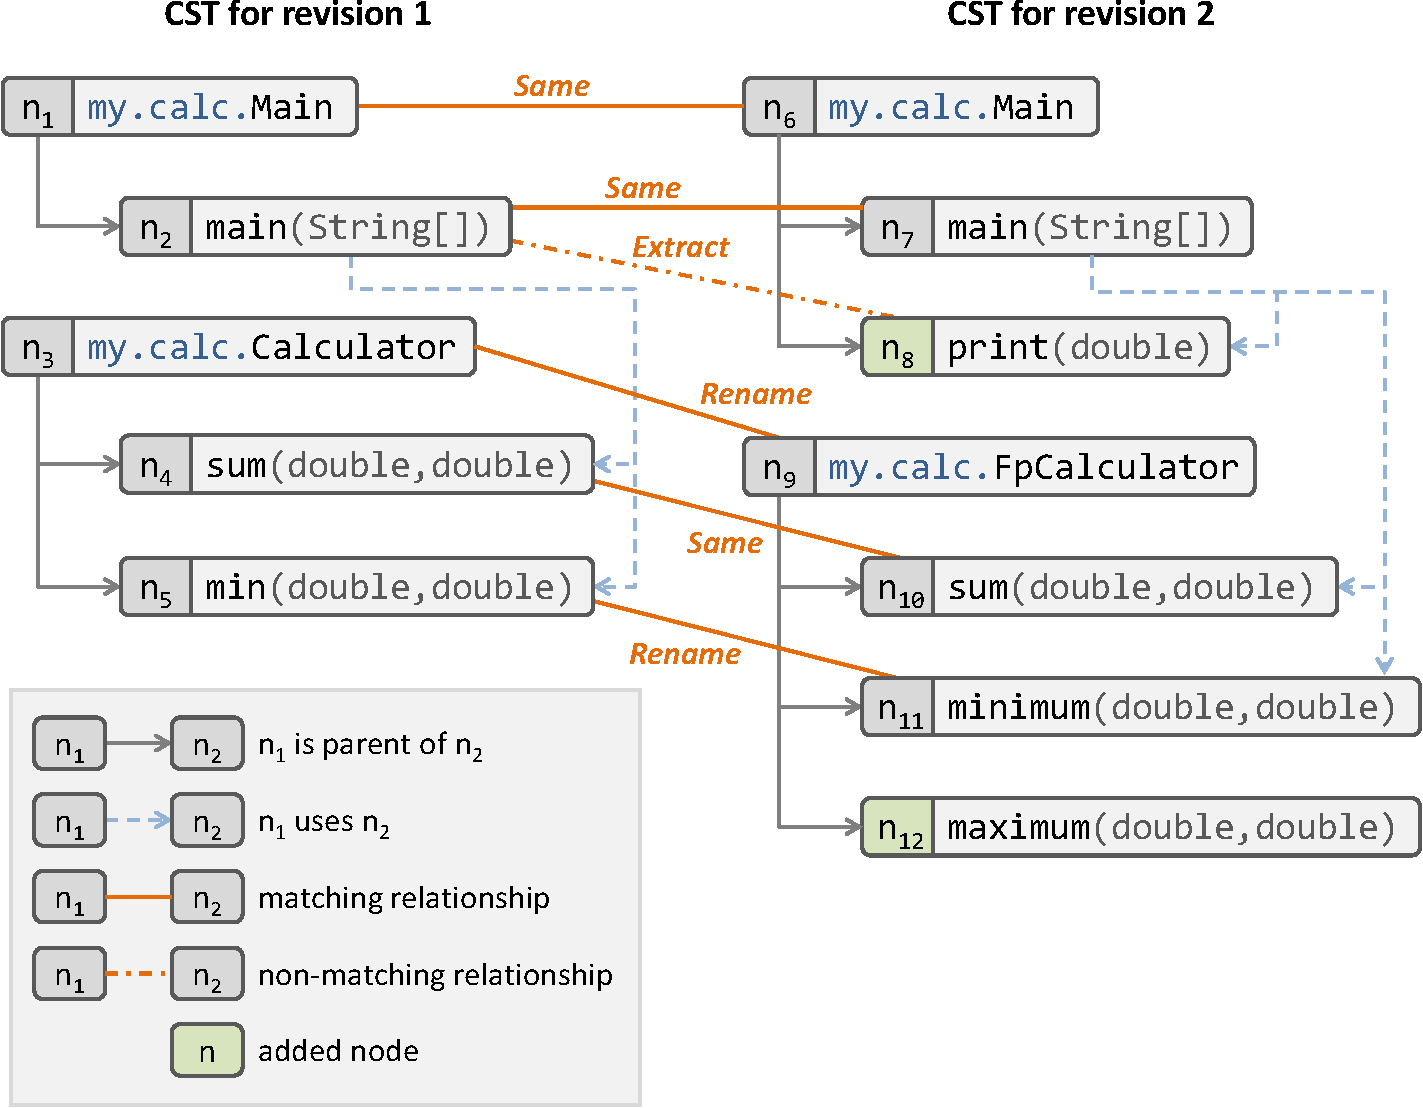
\includegraphics[width=0.75\linewidth]{img/relationshipDiff1.pdf}
\caption{Relationships found in the example from Figure~\ref{FigDiff1}}
\label{FigRelationships1}
\end{figure}


\subsubsection{Dependent and conflicting relationships}
\label{SecDependentConflictingRel}

In some cases, correctly finding a relationship depends on finding a prior relationship.
For example, consider the relationship $(n_5, n_{11}, Rename)$ in Figure~\ref{FigRelationships1} (method \codeinl{min} renamed to \codeinl{minimum}).
The conditions for this relationship includes the clause $\rdparent(n_5)' = \rdparent(n_{11})$, which means that the matching node of the parent of $n_5$ should be equal to the parent of $n_{11}$ (see Table~\ref{TabRelationshipTypes}, \textit{Rename} row).
This clause only yields true after the matching pair $(n_3, n_9)$ is added to $M$, i.e., after we find out that \codeinl{Calculator} is renamed to \codeinl{FpCalculator}.
In fact, if we call $\mathit{findMatchRel}(n_5, n_{11})$ before $M$ contains $(n_3, n_9)$, we would incorrectly classify it as a \textit{Move and Rename} relationship.
To address this issue, we only resolve the actual relationship types in steps~4 and~5, after all matching pairs are found (note that in steps~1, 2, and 3 we record the matching pairs in $M$, purposely ignoring the type of relationship).
%Moreover, non-matching relationships, which also depends on the matchings found, are analyzed in the last step. 

Another issue which we may face when looking for relationships are conflicts, i.e., two or more matching relationships hold for the same code element (according to conditions from Table~\ref{TabRelationshipTypes}).
For instance, in the example from Figure~\ref{FigRelationships1}, the conditions for \textit{Rename} yield true for the pair of methods \codeinl{min} and \codeinl{minimum} because their source code are similar and their parents match.
However, this is also the case for the pair of methods \codeinl{min} and \codeinl{maximum}, whose bodies are also similar.
We cannot match the same node twice, thus, we must decide upon which relationship we will accept and discard the other one.
This issue is addressed in procedures \textsc{findMatchingsBySim} and \textsc{findMatchingsByChildr} by using the $\rdsortbysim$ function to sort the potential matching pairs, enforcing that we take first the most likely matches.
The $\rdsortbysim$ function relies on a similarity metric, which we discuss in details in Section~\ref{SecCodeSim}.
After a matching pair $(n_1, n_2)$ is added to $M$, no more matchings involving $n_1$ or $n_2$ are accepted, because \textsc{addMatch} procedure checks that $n_1 \in N^- \land n_2 \in N^+$ (line~47).







\subsection{Code Similarity}
\label{SecCodeSim}



A key element of our approach to find relationships, as previously mentioned, is computing the similarity between code elements (i.e., CST nodes).
The first step to compute this similarity is to represent their source code as a multiset (or bag) of tokens.
A multiset is a generalization of the concept of a set, but it allows multiple instances of the same element.
The multiplicity of an element is the number of occurrences of that element within the multiset.
This representation provides two advantages for our approach.
First, it makes the CST simpler and less coupled to the syntax of programming languages, because we do not need to represent each statement (or AST node) from the source code. Second, we can apply set operations to the bag of tokens, such as subtraction, which is important to detect \emph{Extract} relationships, as we will discuss in Section~\ref{SecSimX}.

Formally, a multiset can be defined in terms of a multiplicity function $m: U \to \mathbb{N}$, where $U$ is the set of all possible elements. In other words, $m(t)$ is the multiplicity of the element $t$ in the multiset. Note that the multiplicity of an element that is not in the multiset is zero.
For example, Figure~\ref{FigSourceCodeTransformation} depicts the transformation of the source code of three methods (\codeinl{sum}, \codeinl{min}, and \codeinl{power}), of the class \codeinl{Calculator}, into multisets of tokens. In this figure, the multiplicity function $m$ for each method is represented in a tabular form. For example, the multiplicity of the token \codeinl{y} in method \codeinl{min} is two (i.e., $m_{\mathtt{min}}(\mathtt{y}) = 2$), whilst the multiplicity of the token \codeinl{if} in method \codeinl{power} is zero (i.e., $m_{\mathtt{power}}(\mathtt{if}) = 0$).

\begin{figure*}[tbp]
\renewcommand{\arraystretch}{1.2}
\centering
\footnotesize
\resizebox{\columnwidth}{!}{%
\begin{tabular}{@{}llll@{}}
\begin{tabular}{p{8cm}}
\multicolumn{1}{c}{\textbf{Source code of a class}} \\
\begin{lstlisting}
public class Calculator {

  public int sum(int x, int y) {
    return x + y;
  }

  public int min(int x, int y) {
    if (x < y) return x;
    else return y;
  }

  public double power(int b, int e) {
    return Math.pow(b, e);
  }
}
\end{lstlisting}\\

\end{tabular}
& {\Large $\Rightarrow$} &
\begin{tabular}{|l|r|r|r|}
\multicolumn{4}{c}{\textbf{Multiset of tokens for each method}} \\
\hline
Token $t$ & $m_{\mathtt{sum}}(t)$ & $m_{\mathtt{min}}(t)$ & $m_{\mathtt{power}}(t)$\\
\hline
\codeinl{return} & 1 & 2 & 1 \\
\codeinl{x}      & 1 & 2 & 0 \\
\codeinl{+}      & 1 & 0 & 0 \\
\codeinl{y}      & 1 & 2 & 0 \\
\codeinl{;}      & 1 & 2 & 1 \\
\codeinl{if}     & 0 & 1 & 0 \\
\codeinl{(}      & 0 & 1 & 1 \\
\codeinl{<}      & 0 & 1 & 0 \\
\codeinl{)}      & 0 & 1 & 1 \\
\codeinl{else}   & 0 & 1 & 0 \\
\codeinl{Math}   & 0 & 0 & 1 \\
\codeinl{.}      & 0 & 0 & 1 \\
\codeinl{pow}    & 0 & 0 & 1 \\
\codeinl{b}      & 0 & 0 & 1 \\
\codeinl{,}      & 0 & 0 & 1 \\
\codeinl{e}      & 0 & 0 & 1 \\
\hline
\end{tabular} &
\begin{tabular}{|r|}
\multicolumn{1}{c}{} \\
\hline
$n_t$\\
\hline
3 \\
2 \\
1 \\
2 \\
3 \\
1 \\
2 \\
1 \\
2 \\
1 \\
1 \\
1 \\
1 \\
1 \\
1 \\
1 \\
\hline
\end{tabular}
\end{tabular}
}
\caption{Transformation of the body of methods into a multiset of tokens}
\label{FigSourceCodeTransformation}
\end{figure*}

After extracting a multiset of tokens, we also compute a weight for each token
of the source code.
In fact, some tokens are more important than others to discriminate a code element.
For example, in Figure~\ref{FigSourceCodeTransformation}, all three methods contain the token \codeinl{return}. In contrast, only one method (\codeinl{power}) contains the token \codeinl{Math}. Therefore, the later is a better indicator of similarity between methods than the former.

In order to take this into account, we employ a variation of the TF-IDF weighting scheme~\citep{salton1986introduction}, which is a well-known technique from information retrieval.
TF-IDF, which is the short form of \emph{Term Frequency-Inverse Document Frequency}, reflects how important a term is to a document within a collection of documents.
In the context of code elements, we consider a token as a term, and a code element as a document.
Let $E$ be the set of all code elements and $n_t$ be the number of elements in $E$ that contains the token $t$. The Inverse Document Frequency ($\mathit{idf}$), is defined as:
\begin{align}
\mathit{idf}(t) = \log (1 + \frac{|E|}{n_t})
\end{align}

Note that the value of $\mathit{idf}(t)$ decreases as $n_t$ increases, because the more frequent a token is among the collection of code elements, the less important it is to distinguish them.
For example, in Figure~\ref{FigSourceCodeTransformation}, the token \codeinl{y} occurs in two methods (\codeinl{sum} and \codeinl{min}). Thus, its $\mathit{idf}$ is:

\[
\mathit{idf}(\mathtt{y}) = 
\log (1 + \frac{|E|}{n_t}) = 
\log (1 + \frac{3}{2}) = 0.398
\]

On the other hand, the token \codeinl{else} occurs in one method ($\mathtt{min}$), and therefore its $\mathit{idf}$ is:

\[
\mathit{idf}(\mathtt{else}) = 
\log (1 + \frac{|E|}{n_t}) = 
\log (1 + \frac{3}{1}) = 0.602
\]

Last, to compute the similarity between two code elements $e_1$ and $e_2$, we use a generalization of the Jaccard coefficient, known as weighted Jaccard coefficient~\citep{chierichetti2010finding}.
Let $U$ be the set of all possible tokens and $m_i: U \to \mathbb{N}$ be the multiplicity function representing the multiset of tokens of a code element $e_i$.
We define the similarity between $e_1$ and $e_2$ by the following formula:


\begin{align}
\label{WJaccard}
\rdsim(e_1, e_2) = \frac{\sum_{t \in U} \min(m_1(t), m_2(t)) \times \mathit{idf}(t) }
                        {\sum_{t \in U} \max(m_1(t), m_2(t)) \times \mathit{idf}(t) }
\end{align}

The rationale behind this formula is that the similarity is at maximum (1.0) when the multiset of tokens representing $e_1$ and $e_2$ contain the same tokens with the same cardinality. In contrast, if the multisets contain no tokens in common, the similarity is zero. Additionaly, tokens with higher $\mathit{idf}$ will have a higher weight.
%It is worth noting that when both multisets are empty, the denominator of the formula is zero, which yields undefined. We handle such special case considering that the similarity is zero.


\subsubsection{Name similarity}
\label{SecNameSim}

Besides relying on the code similarity, our algorithm also depends on the function $\rdnsim(n_1, n_2)$ in Step~3.
This function denotes the similarity between the names of the code elements $n_1$ and $n_2$.
For computing $\rdnsim$, we first decompose the identifiers of $n_1$ and $n_2$ into their composing words. Specifically, we split camel case (e.g., \codeinl{myIdentifier}) or snake case patterns (e.g., \codeinl{my\_identifier}) . For example, \codeinl{SomeLong\_Name} yields three terms: \codeinl{Some}, \codeinl{Long}, and \codeinl{Name}.
Then, we compute $\rdnsim$ using the same formula from $\rdsim$ (see Equation~\ref{WJaccard}), but in this case, each multiset of tokens contains the terms composing the identifiers of $n_1$ and $n_2$.


\subsubsection{Extract similarity}
\label{SecSimX}

While the similarity function $\rdsim$ presented previously is suitable to compute whether two code elements are similar, it is not appropriate to assess whether a code element is extracted from another one, because their source code may be significantly different on their entirety.
However, if a method $e_2$ is extracted from $e_1$, we expect that part of the code of $e_1$ is moved to $e_2$.
Therefore, the source code of the body of $e_2$ should be similar to the source code removed from $e_1$.
Additionally, not all code removed from $e_1$ may have been moved to $e_2$, i.e., some parts of the code may have been extracted to other locations or simply deleted.
To be less susceptible to this issue, our similarity index for \textit{Extract} relationships rely on the following assumption: the code from the body of $e_2$ should be mostly contained in the code removed from $e_1$.

%However, we face two issues when directly comparing the code removed from $e_1$ with the body of $e_2$. First, not all code removed from $e_1$ may have been moved to $e_2$, i.e., some parts of the code may have been extracted to other locations or simply deleted. Second, $e_2$ may contain additional code, introduced after the extraction. In fact, one of the common reasons to extract a method/function is to facilitate the addition of new code~\cite{fse2016-why-we-refactor}. Thus, to be less susceptible to those issues, our similarity index for \textit{Extract} relationships relies on two heuristics: (i) the code from the body of $e_2$ should be mostly contained in the code removed from $e_1$, or (ii) the code removed from $e_1$ should be mostly contained in the body of $e_2$.

Thus, to compute the extract similarity, first we need to compute the code removed from $e_1$. As we represent the source code as multisets of tokens, we are able to use the subtract operation to achieve this goal.
Let $m_1$ be the multiset of tokens of $e_1$ before the change and $m_1'$ be the multiset of tokens of $e_1$ after the change.
The subtract operation between both multisets, which we denote by $m_1' \setminus m_1$, yields a new multiset $m_1^-$ defined by the following multiplicity function:
\begin{align}
m_1^-(t) = \max(0, m_1'(t) - m_1(t))
\end{align}

Besides computing the code removed from $e_1$, we need to measure if it is contained within $e_2$. Thus, we employ a variation of the weighted Jaccard coefficient introduced previously (see Equation~\ref{WJaccard}), which is defined as:
\begin{align}
\rdsimc(m_1, m_2) = \frac{\sum_{t \in U} \min(m_1(t), m_2(t)) \times \mathit{idf}(t)}
                        {\sum_{t \in U} m_1(t) \times \mathit{idf}(t)}
\end{align}
where $m_1$ and $m_2$ are multisets (defined by their multiplicity functions).
In this variation, we change the denominator of Equation~\ref{WJaccard} to include only the multiplicity of the tokens from the first multiset (not their union).
This way, the similarity is at maximum (1.0) when $m_1$ is a subset of $m_2$, even if both multisets are not identical. In contrast, the similarity is zero when the intersection between $m_1$ and $m_2$ is empty.


Given these definitions, we are able to define the extract similarity index, $\rdsimx$, as:
\begin{align}
%\rdsimx(e_1, e_2) = \max( \rdsimc(m_1^-, m_2), \rdsimc(m_2, m_1^-) )
\rdsimx(e_1, e_2) = \rdsimc(m_2, m_1^-)
\end{align}
where $m_1^-$ is the multiset representing the code removed from $e_1$ ($m_1 \setminus m_1'$) and $m_2$ is the multiset representing the source code of the body of $e_2$.
The rationale behind this formula is that the similarity is at maximum
%when $m_1^-$ is a subset of $m_2$, or 
when $m_2$ is a subset of $m_1^-$, addressing the previously described heuristic.
%that the code from the body of $e_2$ should be mostly contained in the code removed from $e_1$.



%When building the multiset of tokens representing the source code of the body of a code element, we ignore any occurrence of identifiers that are parameters. 

\subsubsection{Inline similarity}
\label{SecSimI}

The similarity index for computing \textit{Inline} relationships is analogous to the \textit{Extract} similarity index.
%, but we adopt a simpler heuristic in this instance because it is less common to introduce code changes in the inlined method along with the refactoring operation \todo{esta explicacao nao tem muito fundamento na verdade}.
If a code element $e_1$ is inlined into a code element $e_2$, we expect that the code from the body of $e_1$ should be mostly contained in the code added to $e_2$. Specifically, we define the inline similarity index, $\rdsimi$, as:
\begin{align}
\rdsimi(e_1, e_2) = \rdsimc(m_1, m_2^+)
\end{align}
where $m_1$ is the multiset representing the source code of the body of $e_1$ and $m_2^+$ is the multiset representing the code added to $e_2$ ($m_2' \setminus m_2$). Such similarity index is at maximum (1.0) when $m_1$ is a subset of the added code ($m_2^+$).





\subsubsection{Ignoring parameters and return keywords}
\label{SecIgnoringReturn}

%\noindent\textbf{Ignoring parameters and \codeinl{return} keywords}\\
When retrieving the tokenized source code of the body of a code element, some tokens are ignored to avoid that syntactical constructs necessary to its declaration
introduce noise when computing the \textit{Extract} or \textit{Inline} similarity index.
For example, suppose we take the refactoring operation \#1 depicted in Figure~\ref{FigDiff1}: \codeinl{print} is extracted from \codeinl{main}.
The body of the new method \codeinl{print} contains a single statement:
\begin{lstlisting}
System.out.printf("%.2f", res);
\end{lstlisting}
All the tokens within this method are present in \codeinl{main} before the extraction, except the identifier \codeinl{res}, which is a declared parameter of \codeinl{print}. In fact, in the original statement, a variable \codeinl{r} is used in place of \codeinl{res}. To be less susceptible to such differences, we omit all occurences of parameters in the tokenized source code of the body. Similarly, occurences of \codeinl{return} keywords are also ignored because they may be introduced when turning the extracted code into a method.
It is worth noting that discarding such tokens is of responsability of the source analysis module. Thus, specific rules may be implemented according to the peculiarities of the programming language.


\subsection{Implementation details}

RefDiff implementation consists of a core module and language plugins:

\begin{itemize}
\item \textbf{\texttt{refdiff-core}}: implements our core algorithm and contains common data types to represent CSTs and interfaces to implement source code analysis (i.e., generation of CSTs) for each programming language. Currently, this module contains 3,103 lines of code, implemented in Java.

\item \textbf{\texttt{refdiff-java}}: language plugin for Java, which relies on the Eclipse JDT library for parsing and analyzing Java code.\footnote{\url{https://www.eclipse.org/jdt/}}
This module contains 1,137 lines of code.
\item \textbf{\texttt{refdiff-c}}: language plugin for C, using the Eclipse CDT library.\footnote{\url{https://www.eclipse.org/cdt/}}
This module contains 615 lines of code.
\item \textbf{\texttt{refdiff-js}}: language plugin for JavaScript, using the Babel parser\footnote{\url{https://babeljs.io/docs/en/babel-parser}}
and with 689 lines of code.
\end{itemize}
To add support to a new programming language, one must implement the  \codeinl{LanguagePlugin} interface, which defines two methods: \codeinl{parse}, which builds the CST given a set of source files, and \codeinl{getAllowedFilesFilter}, which returns an object with a list of allowed file extensions and an optional list of ignored file name suffixes. For example, \textbf{\texttt{refdiff-js}} ignores file names that end with \texttt{.min.js}, which are usually generated code.

When compared to existing refactoring detection approaches, RefDiff's design has the advantage of being loosed coupled to the syntax of Java (and of any other programming language).
For example, RMiner, which is a Java-based approach, relies on a statement matching algorithm and applies two techniques to enable matching of statements that are not textually identical: Abstraction and Syntax-aware replacements of AST nodes~\citep{tsantalis2018rminer}.
Both techniques manipulate syntactic constructs of the Java language,
such as return statements, variable declarations, assignments, method invocations, conditional statements, class instantiations, types, literals, operators, and others. Thus, when adapting these techniques to other programming language, tool builders should carefully consider its particular syntactic constructs. On the other hand, RefDiff's similarity comparison is based on tokenized code. Therefore, it does not depend on the AST nodes of any given language. 
As another example, Java code is structured with classes, which contains methods and attributes, and RMiner detection rules are tightly based on this structure. In contrast, JavaScript code contains functions inside functions with arbitrary levels of nesting. RefDiff is able to deal with both languages because CSTs do not assume any particular hierarchical structure between different types of nodes.

In summary, we do not claim that existing approaches cannot not be extended to other languages, but that would require a non-trivial effort.
By making fewer assumptions about the syntax of the target language we facilitate multi-language support. Note that the implemented language plugins have small code bases (between 615--1137 lines of code).











\section{Evaluation with Java Projects}
\label{sec:eval:java}

In this section, we evaluate the precision and recall of our approach using a recently proposed dataset of refactorings performed in real-world Java open-source projects. We also compare RefDiff's accuracy with RMiner---the current state-of-the-art tool for detecting refactorings in Java---and RefDiff~1.0, the previous version of our tool.
First, we present our evaluation design (Section~\ref{sec:eval:java:design}) and then we present the results (Section~\ref{sec:eval:java:results}).

\subsection{Evaluation Design}
\label{sec:eval:java:design}

To evaluate the precision and recall of RefDiff in Java we initially use an oracle proposed by \cite{tsantalis2018rminer}.
This oracle includes 3,188 manually-validated refactoring instances, detected in 538 commits from 185 open-source projects, and covering 15 refactoring types.
It is important to emphasize that most commits contain non-refactoring changes interleaved with refactorings, which is the most challenging scenario for refactoring detection tools.
In our evaluation, we also compare RefDiff's precision and recall against RMiner.
For the purpose of the comparison, we restricted the oracle to 11 refactoring types supported by both tools.
Specifically, we excluded \emph{Change Package}, \emph{Move Field}, \emph{Push Down Field} and \emph{Pull Up Field} from the analysis as they are not supported by RefDiff.
Moreover, \emph{Convert Type} and \emph{Change Signature}, although supported by RefDiff, are not evaluated because they are not covered by the oracle.
In total, our modified oracle contains 3,031 confirmed refactoring instances.
Additionally, it also contains 704 refactoring instances classified as false positives in the process of manual validation performed by \cite{tsantalis2018rminer}.
These instances are used to detect false positives reported by RefDiff, as described in the next paragraph.
%Last, it is worth noting that the \emph{Rename Class} category also includes instances of \emph{Move and Rename Class}. Similarly, the \emph{Extract Method} category also includes instances of \emph{Extract and Move Method}. This measure was necessary because the oracle did not distinguish between those refactorings reliably.

First, we run RefDiff on each commit of the oracle. For each detected refactoring $r$ we checked whether $r$ is in the oracle, which may yield three outcomes: (i) if $r$ is a confirmed refactoring from the oracle, then it is a true positive; (ii) if $r$ is a false refactoring from the oracle, then it is a false positive; (iii) otherwise, $r$ was inspected by two authors of this paper to assess whether it is a false positive or a true positive not covered by the oracle.
This extra manual validation is needed because the initial oracle must not be granted as complete, i.e., including all refactorings performed in the set of analysed commits.
Specifically, it was constructed using a triangulation approach, based on an initial list of refactorings produced by RMiner and RefDiff~1.0. For this reason, it might miss true refactorings only detected by RefDiff~2.0. %the improved implementation of RefDiff, described in this paper.

%\begin{figure*}[!t]
%\centering
%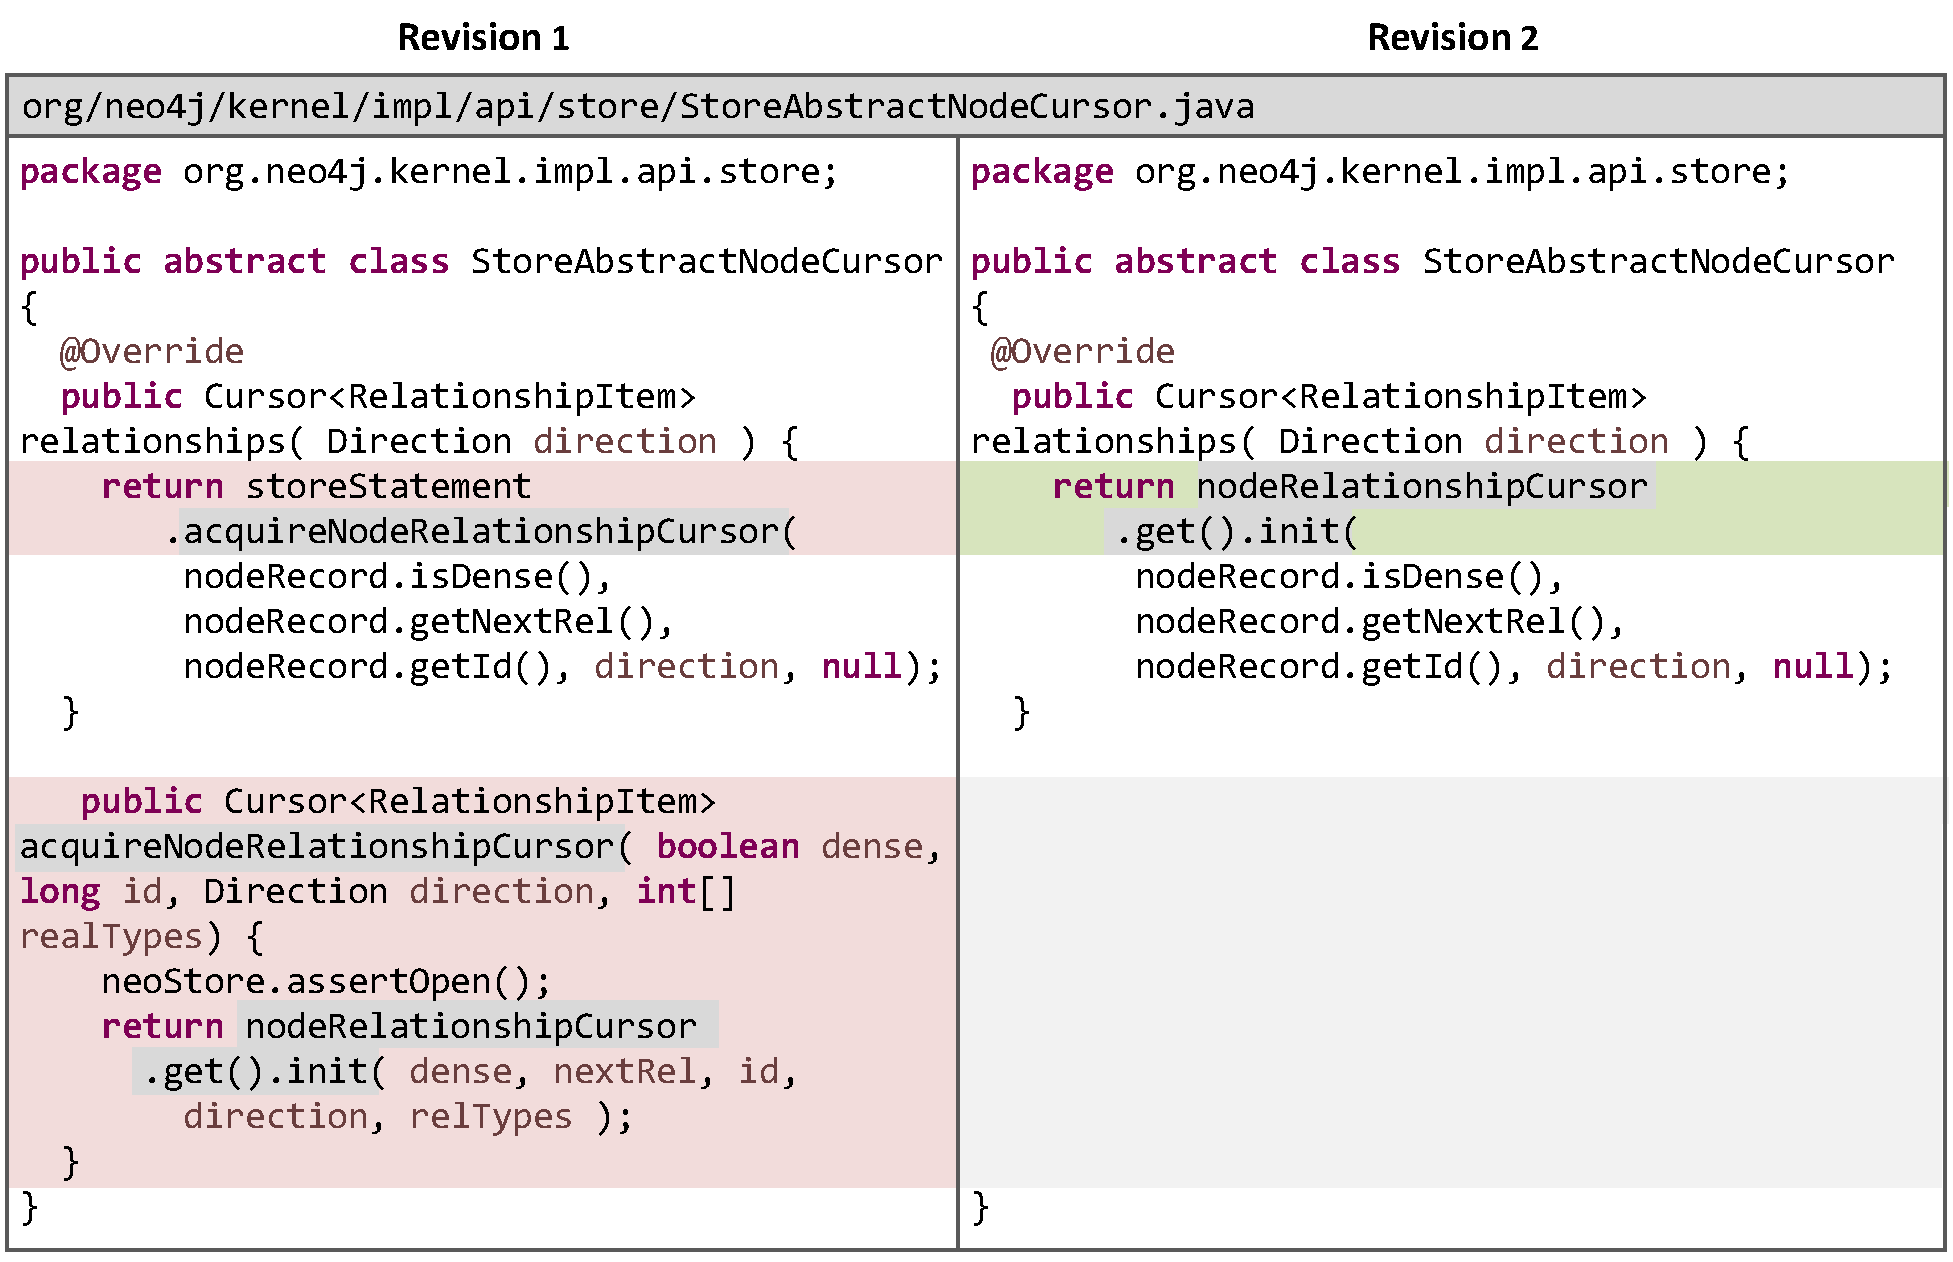
\includegraphics[width=0.8\textwidth]{img/diff2.pdf}
%\caption{Illustrative diff of an \emph{Inline Method} refactoring considered as true positive by the validators.}
%\label{FigDiff2}
%\end{figure*}





After following this procedure, RefDiff 2.0 detected 263 new refactoring instances (i.e., not listed in the initial oracle), which were validated by two paper's authors, called here validators. In the case of 175 refactorings (66\%), the validators agreed on their classification, including 138 refactorings labelled as true positives by both validators and 37 labelled as false positives. After this initial and independent validation, the validators discussed together the remaining 88 cases (34\%), to reach an agreement. As a result, 79 refactorings were considered true positives and 9 refactorings were classified as false positives.
%Figure~\ref{FigDiff2} shows a first example of true positive. RefDiff identified an \emph{Inline Method} refactoring, consisting on the substitution of the method named \codeinl{acquireNodeRelationshipCursor}, which was removed in the same commit, by invocations to methods \codeinl{get()} and \codeinl{init()}. We emphasize in this figure the changes that correspond to this refactoring. This indication of refactoring was not listed in the oracle. The validators individually analyzed this commit and both agreed that an \emph{Inline Method} was applied in this commit.
Figure~\ref{FigDiff3} shows an example of a refactoring identified by RefDiff that both validators classified as true positive.
In this case, a developer extracted method \codeinl{createPrepareRpcOptions} from method \codeinl{prepareOnAffectedNodes}.
%Figure~\ref{FigDiff3} shows an example of a true positive, in which RefDiff identifies a \emph{Extract and Move Method} refactoring. Developers removed the invocation to the method \codeinl{readValue(String, Class)}, which was extracted and moved to the class \codeinl{Controls}. An invocation to this new method \codeinl{validateControlsString(String)} was replaced in the same line.
%Similarly to the example in Figure~\ref{FigDiff2},
%Both validators agreed that \emph{Extract and Move Method} were applied in this commit.
%After the manual validation of the refactoring instances it was possible to identify some common causes of failure.
%In particular, one common reason for \emph{Move Method} false positives was missed \emph{Move/Rename Class}, i.e., RefDiff did not detect that the entire class has been moved (or renamed), and incorrectly reported that several of its members were moved.
%We mitigated this issue by introducing a specific heuristic for this case (see Section~\ref{AlgoGeneral}).
%Moreover, the analysis of the incorrect reports allowed us to identify and fix a couple of bugs in our implementation.
%After applying the aforementioned fixes to RefDiff, it was necessary to run it again and compare the results against the update oracle. This time, 51 new refactoring instances were found, which were  validated by one of the authors. 24 of them (47\%) were classified as true positive, whilst 27 of them (53\%) were classified as false positive.

In total, after completing the manual validation, 217 new refactorings instances were classified as true positives and therefore included in the oracle.
The expanded oracle includes 3,248 refactoring instances (7.19\% more than the initial one) and it is publicly available at RefDiff's GitHub repository.\footnote{\url{https://github.com/aserg-ufmg/RefDiff}}


\begin{figure*}[htpb]
\centering
%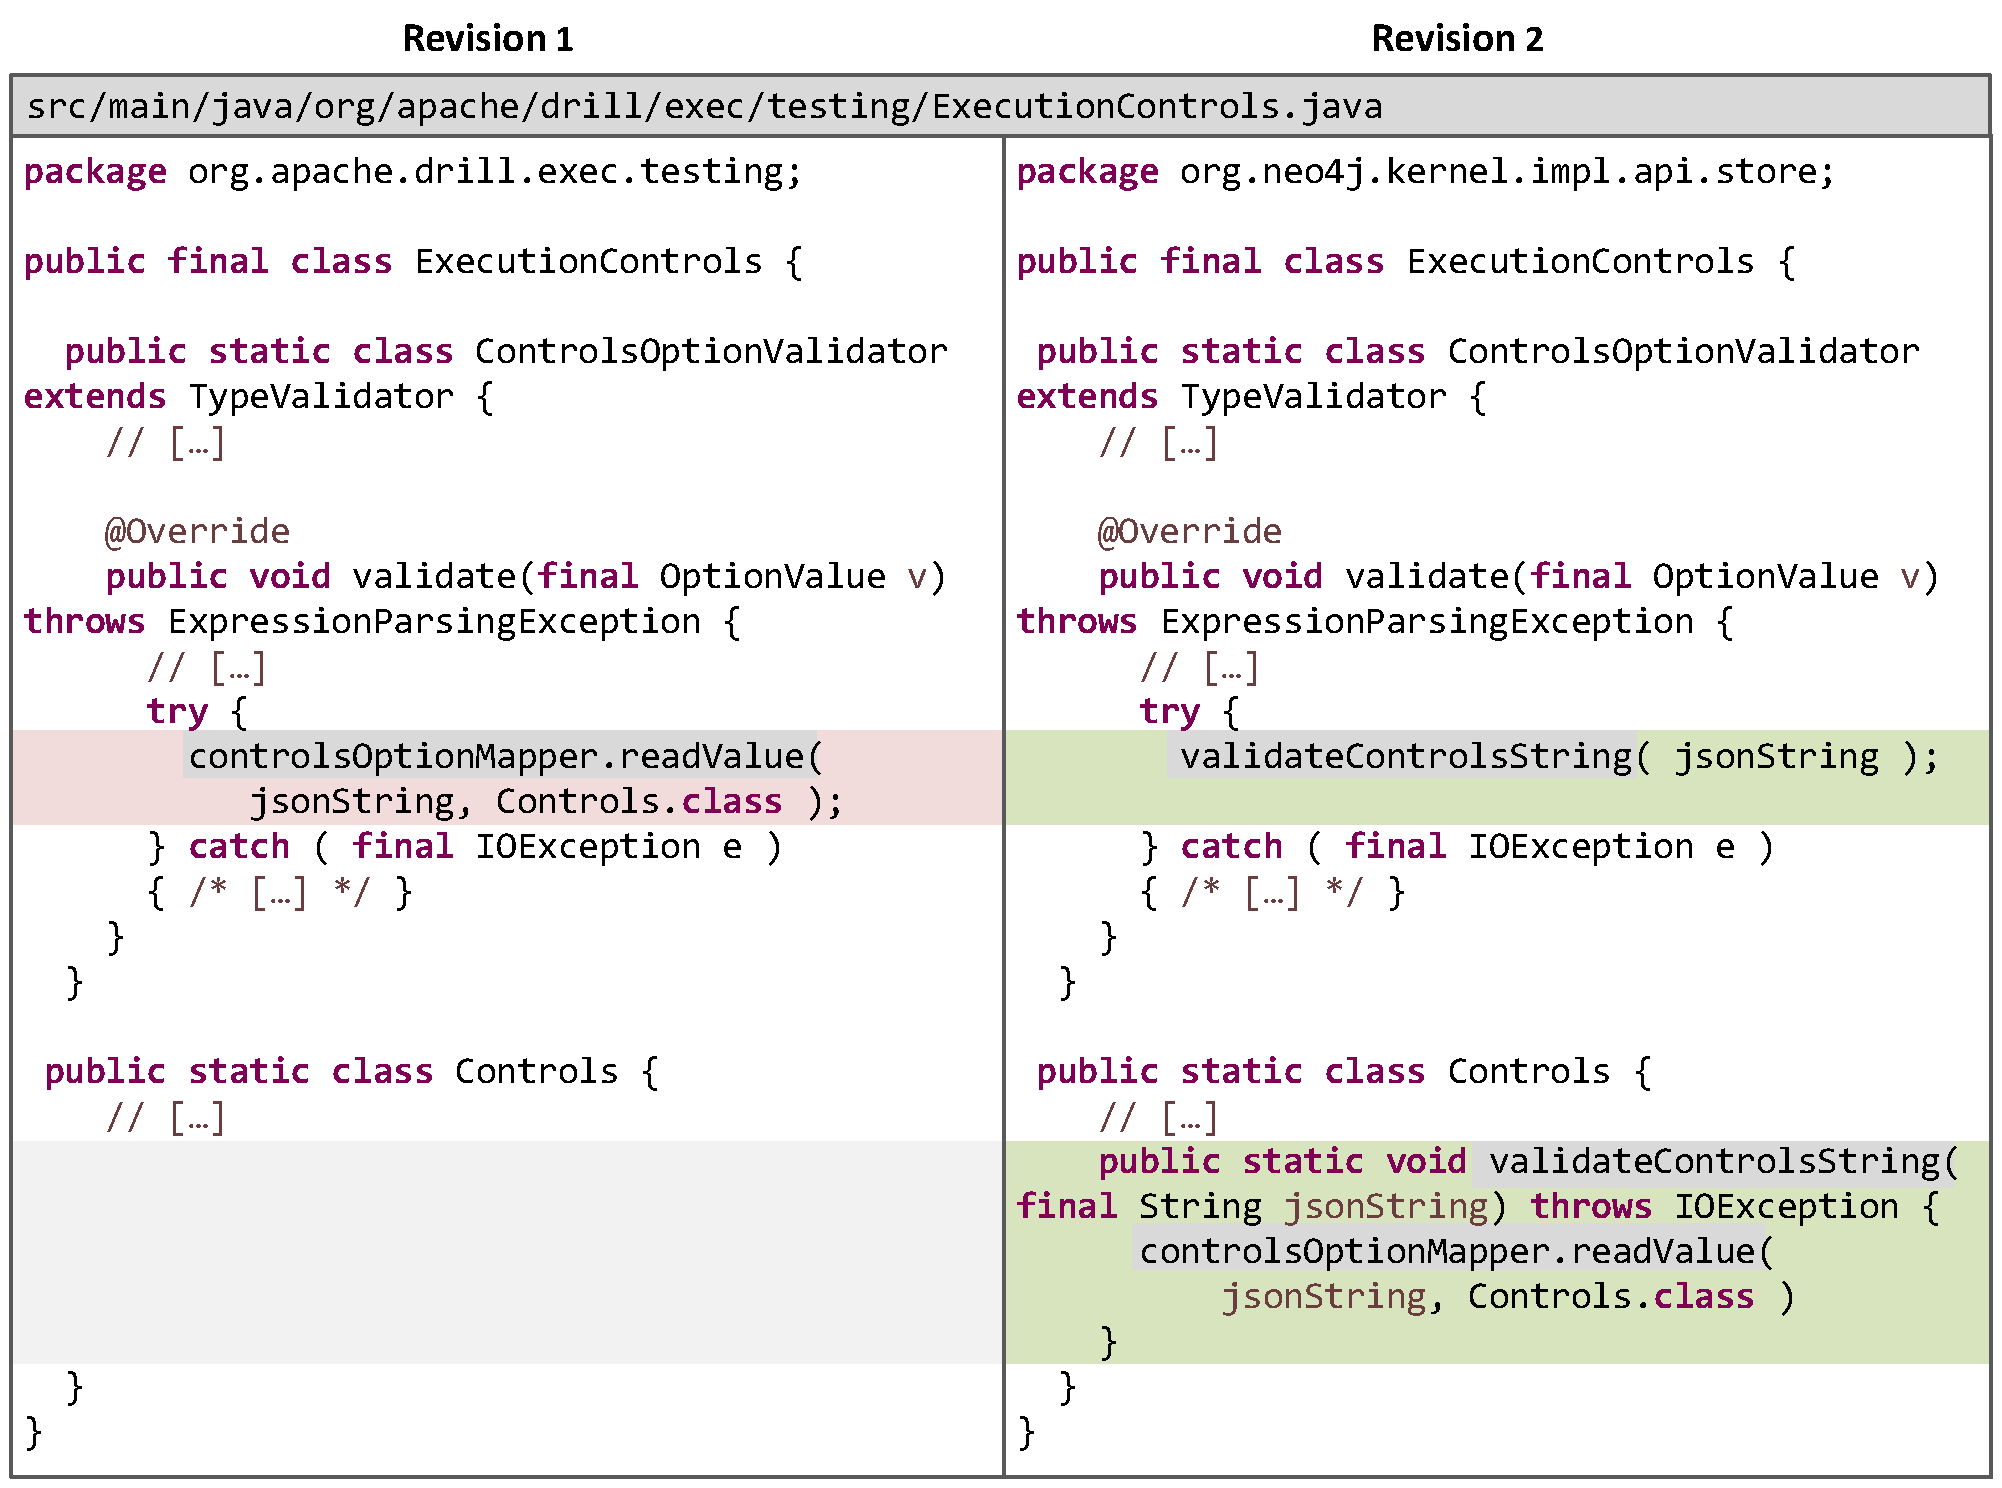
\includegraphics[width=0.8\textwidth]{img/diff3.pdf}
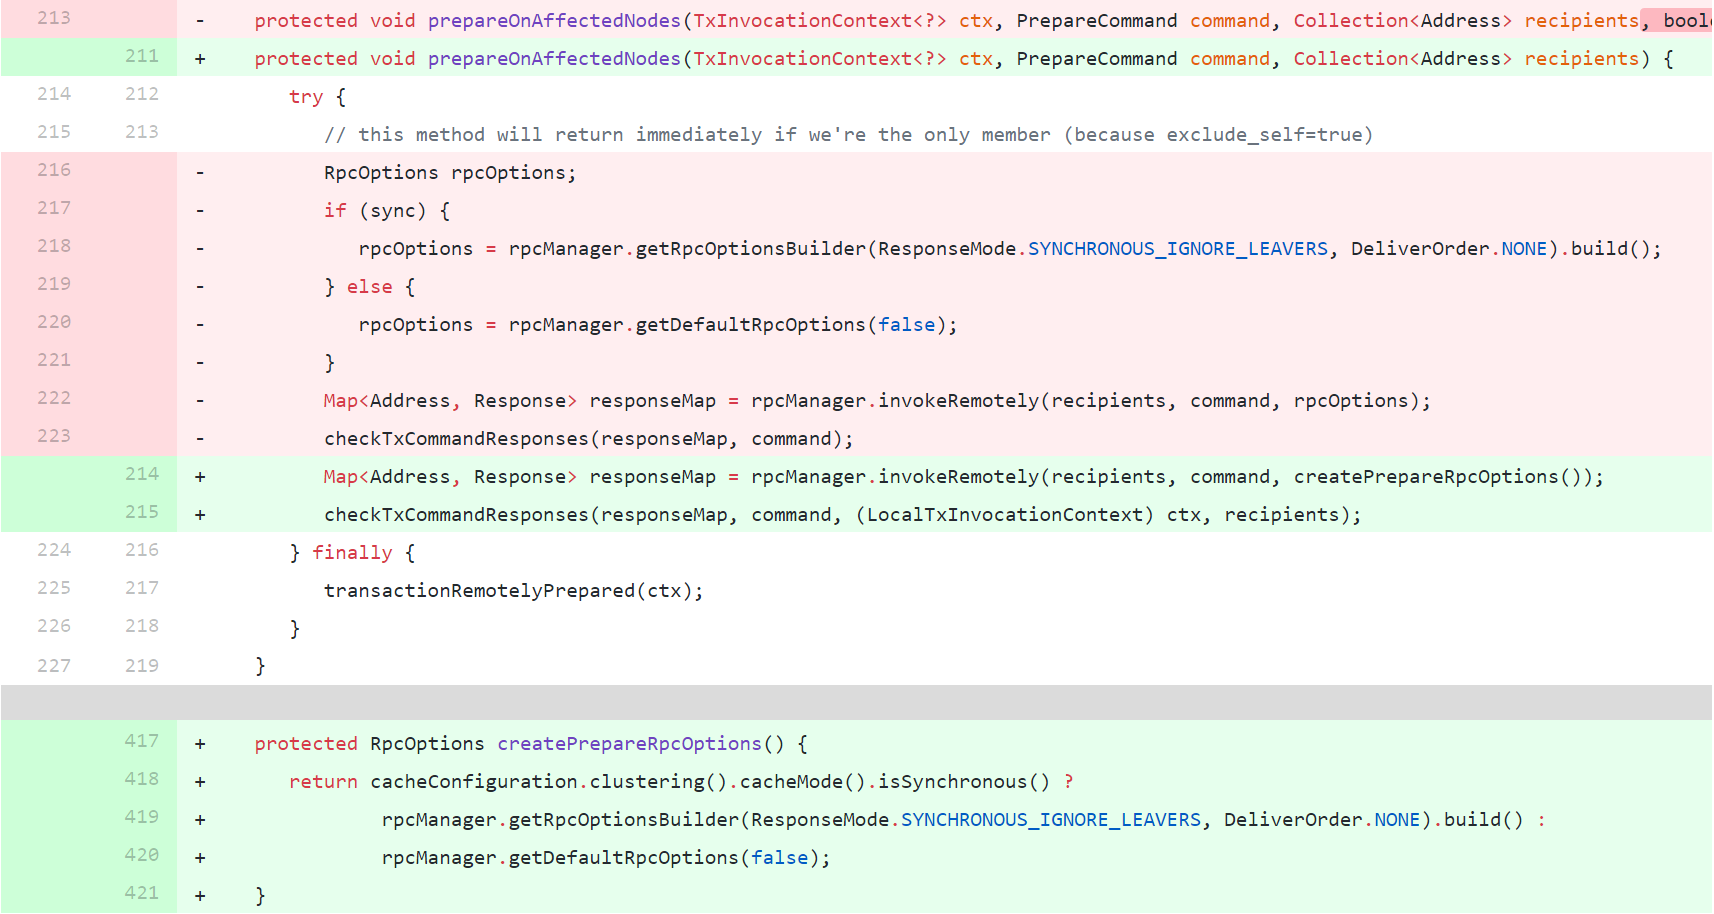
\includegraphics[width=1.0\textwidth]{img/ex-new-extract-infinispan-ce4f629.png}
\caption{Illustrative diff of an \emph{Extract Method} refactoring considered as true positive by the validators, taken from commit ce4f629 from \emph{infinispan} project.}
\label{FigDiff3}
\end{figure*}



\subsection{Results}
\label{sec:eval:java:results}

\begin{table*}[htbp]
\renewcommand{\arraystretch}{1.2}
\caption{Java precision and recall results}
\label{TabResultJava}
\centering
\resizebox{\columnwidth}{!}{%
\begin{tabular}{@{}lrr@{}ll@{}p{0.5cm}@{}ll@{}p{0.5cm}@{}ll@{}}
\toprule
 & & & \multicolumn{2}{c}{RefDiff 1.0} & & \multicolumn{2}{c}{RefDiff 2.0} & & \multicolumn{2}{c}{RMiner}\\
\cmidrule{4-5} \cmidrule{7-8} \cmidrule{10-11}
Refactoring Type & \# & & Precision & Recall & & Precision & Recall & & Precision & Recall \\
\midrule
Move Class & 1100 & & \xbar{0.999} & \xbar{0.881} & & \xbar{0.999} & \xbar{0.970} & & \xbar{1.000} & \xbar{0.925} \\
Move Method & 319 & & \xbar{0.322} & \xbar{0.746} & & \xbar{0.871} & \xbar{0.803} & & \xbar{0.955} & \xbar{0.658} \\
Move and Rename/Rename Class & 95 & & \xbar{0.897} & \xbar{0.642} & & \xbar{0.922} & \xbar{0.874} & & \xbar{0.983} & \xbar{0.621} \\
Rename Method & 350 & & \xbar{0.855} & \xbar{0.811} & & \xbar{0.946} & \xbar{0.694} & & \xbar{0.978} & \xbar{0.771} \\
Extract Interface & 24 & & \xbar{0.769} & \xbar{0.417} & & \xbar{0.875} & \xbar{0.875} & & \xbar{1.000} & \xbar{0.833} \\
Extract Superclass & 70 & & \xbar{1.000} & \xbar{0.157} & & \xbar{1.000} & \xbar{0.743} & & \xbar{0.958} & \xbar{0.971} \\
Pull Up Method & 91 & & \xbar{0.806} & \xbar{0.593} & & \xbar{0.974} & \xbar{0.824} & & \xbar{1.000} & \xbar{0.791} \\
Push Down Method & 40 & & \xbar{0.950} & \xbar{0.475} & & \xbar{0.950} & \xbar{0.950} & & \xbar{1.000} & \xbar{0.825} \\
Extract/Extract and Move Method & 1037 & & \xbar{0.904} & \xbar{0.833} & & \xbar{0.962} & \xbar{0.663} & & \xbar{0.985} & \xbar{0.768} \\
Inline Method & 122 & & \xbar{0.842} & \xbar{0.787} & & \xbar{0.957} & \xbar{0.721} & & \xbar{0.990} & \xbar{0.795} \\
\addlinespace
Total & 3248 & & \xbar{0.792} & \xbar{0.802} & & \xbar{0.964} & \xbar{0.804} & & \xbar{0.988} & \xbar{0.813} \\
\bottomrule
\end{tabular}
}
\end{table*}

Table~\ref{TabResultJava} shows the precision and recall results for RefDiff~2.0 and RMiner using the oracle described in the previous section. The overall precision and recall of RefDiff~2.0 is 96.4\% and 80.4\%, respectively.
Precision ranges from 87.1\% (\emph{Move Method}) to 100.0\% (\emph{Extract Superclass}), and it is above 90\% for 8 out of 10 refactoring types.
Recall ranges from 66.3\% (\emph{Extract Method}) to 97.0\% (\emph{Move Class}), and it is above 80\% for 6 out of 10 refactoring types.


\subsubsection{Comparison with RefDiff 1.0}

We also show in Table~\ref{TabResultJava} the results obtained with RefDiff~1.0 in this oracle. Note that overall precision is significantly improved (from 79.2\% to 96.4\%). Moreover, RefDiff~2.0 has less variation on recall across refactoring types.
We can list five improvements over RefDiff 1.0 that justify such results.
\begin{itemize}
\item In RefDiff 2.0, we find moved/renamed types (e.g., classes) based on matched members (step~3 of our algorithm). This heuristic was introduced aiming to reduce the number of false negatives for class moves/renames, which also reduces the number of false positives for \emph{Move Method}.

\item We compute the removed and added code using set operations to improve \emph{Extract} and \emph{Inline} similarity functions. For example, our \emph{Extract} similarity function compares the body of an extracted method with the code removed from the original method, strengthening the preconditions to detect \emph{Extract} relationships. Similarly, our \emph{Inline} similarity function compares the body of an inlined method with the code added to its destination.

\item Ignoring parameters/arguments and return keyword (Section~\ref{SecIgnoringReturn}) is also an improvement over RefDiff~1.0, making \emph{Extract} and \emph{Inline} similarity less sensitive to code changes related to the mechanics of the refactoring.

\item \emph{Pull Up} and \emph{Push Down} rules no longer include body similarity comparison. Additionally, \emph{Extract Supertype} also drops similarity comparison and it was rewritten based on \emph{Pull Up} rule. These changes improved both precision and recall of these refactoring types.

\item While RefDiff 1.0 relied on a set of thresholds, which were calibrated for each refactoring type, in RefDiff 2.0 we use a single similarity threshold, defined as 0.5 by default.
We acknowledged that relying on user-defined thresholds or thresholds calibration is not ideal, as advocated by \cite{tsantalis2018rminer}.
Thus, in RefDiff 2.0 we emphasized the aforementioned improvements to our algorithm, making it is less sensitive to similarity thresholds.
In fact, we achieved better precision for all refactoring types, even without calibration.
We only lost recall for \emph{Rename Method}, \emph{Extract Method} and \emph{Inline Method}.
We attribute this fact to the very low thresholds set for these refactoring types (between 0.1 and 0.3).
%, possibly overfitted to the characteristics of the calibration oracle used in RefDiff 1.0.

\end{itemize}


\subsubsection{Comparison with RMiner}

Table~\ref{TabResultJava} also shows the results of RMiner, which achieves 98.8\% of overall precision (ranging from 95.5\% to 100.0\%) and 81.3\% of overall recall (ranging from 64.1\% to 97.1\%).
When we analyze individual refactoring types, RefDiff's precision is lower in all but one refactoring type (\emph{Extract Superclass}). However, recall is higher in 6 refactoring types.
In summary, both tools have very similar total recall, but RMiner's precision is slightly higher.
We can list at least three differences between RefDiff and RMiner that might explain the differences in the results.
\begin{itemize}

\item Unlike RefDiff, we believe RMiner does not account for methods moved to added classes, nor methods moved from deleted classes, as RMiner's detection rule for \emph{Move Method} includes the clauses $(\mathit{td}_a, \mathit{td}_a') \in TD^=$ and $(\mathit{td}_b, \mathit{td}_b') \in TD^=$~\citep{tsantalis2018rminer}.
Many of the false negatives for \emph{Move Method} involve such scenarios, which explains the lower recall for RMiner.


\item Both approaches find moved/renamed types (e.g., classes) based on matched members (step~3 of our algorithm). However, ReffDiff's detection rule requires that a pair of candidate types $(t_1, t_2)$ have more than one children in common, while RMiner's rule is more strict, requiring that either all members of $t_1$ are in $t_2$, or all members of $t_2$ are in $t_1$.
Additionally, RefDiff also finds moved/renamed types by similarity. 
These might be the reasons for RMiner's lower recall for \emph{Move and Rename/Rename Class}.

\item They use very different approaches for computing code similarity. While RefDiff relies on tokenized code and a TF-IDF based similarity function, RMiner relies on a statement matching algorithm and syntax-aware replacement of AST nodes.
Such difference potentially impacts precision and recall for several refactoring types, and might be an advantage factor for RMiner.
\end{itemize}

Despite the aforementioned differences, we emphasize that RefDiff and RMiner have much in common:
\begin{itemize}
\item Both approaches match elements by full name/signature in their first step.

\item Many of the refactoring detection rules are similar.

\item Both approaches enforce an order of detection between refactoring types and use a best match strategy to choose between conflicting refactoring candidates.
%However, there is a subtle difference. RMiner ranks candidates for each refactoring type individually, while RefDiff ranks candidates for all matching relationships together.
%This means that RMiner will always prefer a local refactoring over a non-local refactoring. In contrast, RefDiff may choose, for example, a \emph{Move} candidate over a \emph{Rename} candidate depending on their similarity score.

\item RefDiff 2.0 included an heuristic to find moved/renamed types (e.g., classes) based on matched members, which is similar to RMiner's detection rule.

\item Ignoring parameters/arguments and return keyword (Section~\ref{SecIgnoringReturn}) serves a similar purpose to the argumentization and abstraction techniques proposed by RMiner.
\end{itemize}


\subsection{Execution time}
\label{SecRefDiffExecTime}

Besides comparing precision and recall, we also compared the execution time of both RefDiff and RMiner.
For this purpose, we ran both tools using the same computer (an Intel Core i5-750 with 8GB of RAM and a 7200 RPM HDD) and measured the time spent in the analysis of each of the 538 commits from our oracle.
Figure~\ref{FigVioplotExecTime} shows a violin plot of the execution time per commit for both tools, using a log-10 scale.
We can note that the median is lower for RMiner (109 ms vs. 157 ms), but RefDiff has less variation in the execution times. For example, the maximum execution time for RMiner was 85s, at commit~ab98bca from  \textit{java-algorithms-implementation}, whilst RefDiff spent 10s at maximum, in commit~4baf0a4 from \textit{aws-sdk-java}.
Nevertheless, both tools analyze the majority of the commits in less than one second and are viable for practical use.
It is worth noting that we executed both RefDiff and RMiner using their file-based API, which  reads a list of files directly from disk.
This means that the time to clone or checkout revisions from git repositories is not included in our measurements.
However, we do not expect significant differences between both tools when using their git-based API, which includes services from mining refactorings directly from git repositories. The reason is that both tools retrieve only the necessary files using the \textit{jgit} library, therefore avoiding checking out the entire project on disk.

\begin{figure}[htbp]
\centering
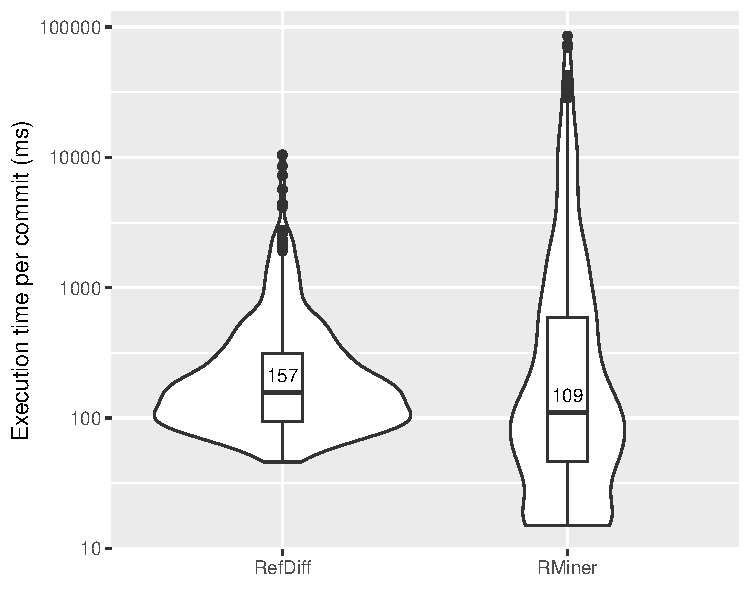
\includegraphics[width=0.7\linewidth]{img/vioplot-exec-time.pdf}
\caption{Violin plot of execution time per commit in log-10 scale}
\label{FigVioplotExecTime}
\end{figure}

\subsection{Threats to Validity}
\label{SecThreatsJava}

There are at least two threats to the validity of the evaluation with Java projects.
The first one is the subjectivity inherent to the manual classification of the reported refactorings as true/false positives, which directly impact the computed precision.
Different validators may have a different interpretation of the code change under analysis, which is demonstrated by the fact that in 34\% of the cases the validators initially disagreed.
We mitigated this threat by having each refactoring assessed by two validators independently.
Second, as discussed in Section~\ref{sec:eval:java:design}, our oracle can not be granted as complete, i.e., there might exist refactorings in the analyzed revisions that are not detected by neither RMiner nor RefDiff.
Thus, the actual recall might be lower than the computed recall.
Unfortunately, it is not feasible to assure the completeness of an oracle at this scale with manual inspection.
A single commit usually contains hundreds of changed lines of code, making such task extremely time consuming and error prone.
Nevertheless, the computed recall serves the purpose of comparison between tools, and it should also be a fair approximation of actual recall, as our oracle is based on refactorings found by three tools: RMiner, RefDiff~1.0, and RefDiff~2.0.

%We cannot claim that the precision and recall of our approach would be the same for different projects, with distinct characteristics, and with actual refactorings applied by developers. However, such setup was necessary to compute recall, as discussed in Section~\ref{SecOracleConstruction}. Besides, the results we achieved in the calibration process (precision of 85.7\% and recall of 94.1\%), in which we used actual commits from relevant Java repositories, suggest that RefDiff's precision and recall are acceptable in real scenarios. Nevertheless, we plan to extend this study by assessing the precision of RefDiff in a large corpus of commits from open-source repositories.
%Neverthless, our evaluation includes relevant Java systems of different domains, with up to 374,000 lines of code.
%, and we have no reasons to  believe that precision and recall will be drastically inferior for other systems.










\section{Evaluation with JavaScript and C}
\label{sec:eval:js:c}

Besides the Java evaluation, we also evaluated precision and recall of RefDiff in JavaScript and C. Unfortunately, we did not find a dataset with detailed information about real refactorings performed in these languages that we could use as an oracle.
Therefore, we had to adopt a different strategy. 
%We also evaluate RefDiff with refactorings performed in two important but very different programming languages: JavaScript (a widely popular dynamic programming language, used mostly to build web applications) and C (a procedural programming language, used mostly to implement system software).
%In the literature, we did not find a dataset with detailed information about real refactorings performed in these languages. Therefore, 
To evaluate precision, we manually validated the refactorings detected by RefDiff in a set of GitHub repositories, in both languages (Section~\ref{sec:eval:js:c:precision}). Then, to evaluate recall, we searched for documented refactoring operations in commit messages of the same set of repositories (Section~\ref{sec:eval:js:c:recall}).
After that, in Section~\ref{sec:eval:js:c:results}, we report the precision and recall achieved by RefDiff.  We are not aware of any other tool for detecting refactorings in these languages. Therefore, in this second evaluation, it was not possible to compare RefDiff's results with competitor tools.


\begin{table*}[htbp]
\renewcommand{\arraystretch}{1.2}
\caption{JavaScript and C repositories used in the evaluation}
\label{TabJsCRepos}
\centering
\resizebox{0.98\columnwidth}{!}{%
\begin{tabular}{@{}lp{13cm}r@{}}
\toprule
Repository & Description & Commits\\
\midrule
react & A declarative, efficient, and flexible JavaScript library for building user interfaces. & 10,964 \\
vue & Vue.js is a progressive, incrementally-adoptable JavaScript framework for building UI on the web. & 3,014 \\
d3 & Bring data to life with SVG, Canvas and HTML. & 4,148 \\
react-native & A framework for building native apps with React. & 16,875 \\
angular.js & AngularJS - HTML enhanced for web apps. & 8,963 \\
create-react-app & Set up a modern web app by running one command. & 2,233 \\
jquery & A fast, small, and feature-rich JavaScript library. & 6,403 \\
atom & The hackable text editor. & 36,752 \\
axios & Promise based HTTP client for the browser and node.js. & 847 \\
three.js & JavaScript 3D library. & 27,762 \\
socket.io & Realtime application framework (Node.JS server). & 1,715 \\
redux & Predictable state container for JavaScript apps. & 2,819 \\
webpack & A bundler for javascript and friends. & 7,852 \\
Semantic-UI & Semantic is a UI component framework based around useful principles from natural language. & 6,684 \\
reveal.js & The HTML Presentation Framework. & 2,341 \\
meteor & Meteor, the JavaScript App Platform. & 21,966 \\
express & Fast, unopinionated, minimalist web framework for node. & 5,555 \\
material-ui & React components for faster and easier web development. & 9,449 \\
Chart.js & Simple HTML5 Charts using the canvas tag. & 2,739 \\
\midrule
linux & Linux kernel source tree. & 839,761 \\
netdata & Real-time performance monitoring, done right! & 8,338 \\
redis & Redis is an in-memory database that persists on disk. & 8,158 \\
git & Git is a free and open-source distributed version control system. & 55,723 \\
ijkplayer & Android/iOS video player based on FFmpeg n3.4, with MediaCodec, VideoToolbox support. & 2,584 \\
php-src & The PHP Interpreter. & 112,847 \\
wrk & Modern HTTP benchmarking tool. & 76 \\
the\_silver\_searcher & A code-searching tool similar to ack, but faster. & 2,016 \\
emscripten & Emscripten: An LLVM-to-Web Compiler. & 19,468 \\
vim & The ubiquitous text editor. & 9,875 \\
jq & Command-line JSON processor. & 1,287 \\
FFmpeg & A complete, cross-platform solution to record, convert and stream audio and video. & 93,898 \\
tmux & A terminal multiplexer: it enables a number of terminals to controlled from a single screen.  & 7,618 \\
nuklear & A single-header ANSI C gui library. & 1,646 \\
obs-studio & Free and open-source software for live streaming and screen recording. & 6,727 \\
libuv & Cross-platform asynchronous I/O. & 4,319 \\
swoole-src & Coroutine-based concurrency library for PHP (like Golang). & 9,938 \\
curl & A command line tool and library for transferring data with URL syntax. & 24,339 \\
toxcore & The future of online communications. & 3,771 \\
darknet & Convolutional Neural Networks. & 436 \\
\bottomrule
\end{tabular}
}
\end{table*}




\subsection{Evaluation Design: Precision}
\label{sec:eval:js:c:precision}


To compute RefDiff's precision when detecting refactorings in JavaScript and C, we followed these steps:

\begin{enumerate}  
\item We selected the 20 most popular GitHub repositories of each language. For this, we queried the GitHub API for repositories, sorting by stars count---which is a reliable indicator of popularity in GitHub~\citep{icsme2016,jss-2018-github-stars} ---and filtering by programming language.
The resulting list of repositories was manually inspected to discard the ones that are not actual software projects, e.g., tutorials or code samples. Then, we forked each selected repository, to preserve their version histories from future changes pushed to the original project. Table~\ref{TabJsCRepos} shows the name, short description, and number of commits of each selected repository, both for JavaScript and C.

\item We ran RefDiff in the version history of each repository. To select the commits, we navigate the commit graph backwards, starting from the most recent commit in the master branch. We also discarded merge commits, i.e.,~commits which have two predecessors. The rationale is that comparing a merge commit with their predecessors results in duplicated reports of refactorings applied in the commits prior to the merge operation. Moreover, to avoid over-representing projects with longer histories, we established a limit of 500 commits per repository. For each selected commit, we compared its source code with its predecessor using RefDiff, to detect refactoring operations.

\item Given the list of refactorings detected by RefDiff, we randomly selected 10 instances of each refactoring type to manually assess whether they correspond to actual refactorings (true positives), or incorrect reports (false positives).
When applying the random selection, we enforced the constraint that we should not select two refactoring instances performed in the same commit.
In this way, we avoid selecting similar refactorings which were performed in batch, e.g., multiple classes or functions moved together.
To confirm each refactoring operation, one of the authors manually inspected the diff of the code changes in the corresponding commit.
\end{enumerate}

After following the three steps, we compute precision as $P = \mathit{TP} / (\mathit{TP} + \mathit{FP})$, where $\mathit{TP}$ is the number of true positives and $\mathit{FP}$ is the number of false positives.



\subsection{Evaluation Design: Recall}
\label{sec:eval:js:c:recall}


To compute RefDiff's recall when detecting refactorings in JavaScript and C, we followed three steps:

\begin{enumerate}  
\item We used GitHub API to find refactorings documented in commits from the repositories selected for evaluating precision (Section~\ref{sec:eval:js:c:precision}). Such queries consist in searching for keywords denoting a particular type of refactoring in the commit message, as described in Table~\ref{TabSearchQueries}. For example, when looking for \emph{Rename Function} refactoring instances, we built a query that looks for commits which contain the keywords \textit{rename} and \textit{function} in their messages, among other combinations.

\item Given the list of results of a query, one of the authors manually inspected each item to assess whether it really contains a refactoring. He started by analyzing the commit message. 
In many cases, the keywords are found in the text, but they are not referring to a refactoring operation.
For example, one of the messages was: \textit{``The routeToRegExp() function, introduced by 840b5f0, could not extract path params if the path contained question mark or hash.''}
This message contains the keywords \textit{extract} and \textit{function}, but clearly does not describe an \emph{Extract Function} refactoring.
In these situations, he discarded the commit with no further analysis.
When the commit message described a refactoring, he checked the code diff to confirm it.
Each confirmed refactoring was recorded in a normalized textual format compatible with the output of RefDiff.
Inspecting the code diff is also necessary to locate the code elements involved in the operation.
For example, the message \textit{``Extract commit phase passes into separate functions''} documents a \emph{Extract Function} refactoring, but does not specify the name of the extracted functions.
He repeated this procedure until he found 10 instances of each refactoring type or when there were no more results to inspect. We found less than 10 instances when looking for \emph{Move and Rename File}, \emph{Move and Rename Function}, and \emph{Inline Function} for JavaScript. Additionally, although modern JavaScript contains classes, we did not find documented refactorings instances of \emph{Move and/or Rename Class}.



% Rename scaledAssetURLScript function to scaledAssetURLNearBundle

%It is worth noting that, during this procedure, most of the results were discarded because the commit message did not actually documented a refactoring. Besides, the diff of some of the commits were so large that could not be displayed in the user interface. In summary, we only registered the refactoring instances that we could confirm both in the commit message and in the code diff.

\item We ran RefDiff in the commits that contain documented and manually-validated refactorings to assess whether they are reported (true positives) or missed (false negatives). 
\end{enumerate}

After following these steps, we compute recall as $R = \mathit{TP} / (\mathit{TP} + \mathit{FN})$, where $\mathit{TP}$ is the number of true positives and $\mathit{FN}$ is the number of false negatives.

\begin{table}[htbp]
\renewcommand{\arraystretch}{1.2}
\caption{Search queries for each refactoring type}
\label{TabSearchQueries}
\centering
\footnotesize
\begin{tabular}{@{}lp{7cm}@{}}
\toprule
%Refactoring Type & Search queries\\
%\midrule
Change Signature & add parameter, remove parameter, add argument \\
\addlinespace
Move/Rename File & move file, rename file, move folder, move rename file, move rename \\
\addlinespace
Move/Rename Function & move function, rename function, move and rename\\
\addlinespace
Extract Function & extract, duplicate, extract function, factor out \\
\addlinespace
Inline Function & inline, inline into, remove indirection, indirect functions, remove wrapper \\
\bottomrule
\end{tabular}
\end{table}

%\subsection{Results}
%\label{sec:eval:js:c:results}

%In this section, we present the precision and recall results for JavaScript (Section~\ref{sec:eval:js:c:results:js}) and C (Section xx).

\subsection{Results for JavaScript and C}
\label{sec:eval:js:c:results}

Table~\ref{TabResultJs} shows the precision and recall results for JavaScript. The overall precision is 91\%. There are three refactorings with precision of 80\%: \textit{Rename Function}, \textit{Move and Rename Function}, and \textit{Inline Function}. For the remaining refactoring types, RefDiff has a precision of 90\% (two refactoring types) or a precision of 100\% (five refactoring types). Table~\ref{TabResultJs} also shows the recall results, which reach 88\% when all refactoring types are considered together.
\textit{Inline function} has the lowest recall (40\%); however, our dataset has only five instances of this operation. There are three refactoring types with recall of 100\%: \textit{Move File}, \textit{Move Function}, \textit{Move and Rename File}. For the other ones, recall ranges between 80\% and 90\%.



%\begin{table}[htbp]
%\renewcommand{\arraystretch}{1.2}
%\caption{JavaScript precision results}
%\label{TabResultJsPrecison}
%\centering
%\begin{tabular}{@{}lrrl@{}}
%\toprule
%Refactoring Type & TP & FP & Precision\\
%\midrule
%Move File & 10 & 0 & \xbar{1.00} \\
%Move Class & 2 & 0 & \xbar{1.00} \\
%Move Function & 9 & 1 & \xbar{0.90} \\
%Rename File & 10 & 0 & \xbar{1.00} \\
%Rename Class & 5 & 0 & \xbar{1.00} \\
%Rename Function & 8 & 2 & \xbar{0.80} \\
%Move and Rename File & 10 & 0 & \xbar{1.00} \\
%Move and Rename Function & 8 & 2 & \xbar{0.80} \\
%Extract Function & 9 & 1 & \xbar{0.90} \\
%Inline Function & 8 & 2 & \xbar{0.80} \\
%\addlinespace
%Total & 79 & 8 & \xbar{0.91} \\
%\bottomrule
%\end{tabular}
%\end{table}

%\begin{table}[htbp]
%\renewcommand{\arraystretch}{1.2}
%\caption{JavaScript recall results}
%\label{TabResultJsRecall}
%\centering
%\begin{tabular}{@{}lrrl@{}}
%\toprule
%Refactoring Type & TP & FN & Recall\\
%\midrule
%Move File & 10 & 0 & \xbar{1.00} \\
%Move Function & 10 & 0 & \xbar{1.00} \\
%Rename File & 8 & 2 & \xbar{0.80} \\
%Rename Function & 9 & 1 & \xbar{0.90} \\
%Move and Rename File & 3 & 0 & \xbar{1.00} \\
%Move and Rename Function & 6 & 1 & \xbar{0.86} \\
%Extract Function & 9 & 1 & \xbar{0.90} \\
%Inline Function & 2 & 3 & \xbar{0.40} \\
%\addlinespace
%Total & 57 & 8 & \xbar{0.88} \\
%\bottomrule
%\end{tabular}
%\end{table}

\begin{table}[htbp]
\renewcommand{\arraystretch}{1.2}
\caption{JavaScript precision and recall results}
\label{TabResultJs}
\centering
\footnotesize
\begin{tabular}{@{}lrllrl@{}}
\toprule
Refactoring Type & \# & Precision & & \# & Recall\\
\midrule
Move File & 10 & \xbar{1.00} & & 10 & \xbar{1.00} \\
Move Class & 2 & \xbar{1.00} & & 0 & \\
Move Function & 10 & \xbar{0.90} & & 10 & \xbar{1.00} \\
Rename File & 10 & \xbar{1.00} & & 10 & \xbar{0.80} \\
Rename Class & 5 & \xbar{1.00} & & 0 & \\
Rename Function & 10 & \xbar{0.80} & & 10 & \xbar{0.90} \\
Move and Rename File & 10 & \xbar{1.00} & & 3 & \xbar{1.00} \\
Move and Rename Function & 10 & \xbar{0.80} & & 7 & \xbar{0.86} \\
Extract Function & 10 & \xbar{0.90} & & 10 & \xbar{0.90} \\
Inline Function & 10 & \xbar{0.80} & & 5 & \xbar{0.40} \\
\addlinespace
Total & 87 & \xbar{0.91} & & 65 & \xbar{0.88} \\
\bottomrule
\end{tabular}
\end{table}



Table~\ref{TabResultC} shows the precision and recall results for C. The overall precision is 88\%. \textit{Inline Function} is the refatoring for which precision is lower (50\%). Besides, there are two refactorings with precision of 80\%: \textit{Move Function} and \textit{Move and Rename Function}. For the remaining refactoring types, RefDiff has a precision of 90\% (one refactoring type) or a precision of 100\% (four refactoring types).
We did not find any instance of \textit{Move and Rename File}, thus we could not compute precision for this refactoring type.
Table~\ref{TabResultC} also shows the recall results, which is 91\% overall.
\textit{Extract Function} (70\%) and \textit{Move Function} (80\%) are the ones with lowest recall.
For the remaining refactoring types, RefDiff has a recall of 90\% (three refactoring types) or a recall of 100\% (four refactoring types).
%It is worth noting that 5 out of 10 false positives we found in our evalution were due to a limitation of our implementation. Currently, the source code analysis plugin for C does not handle preprocessor directives and macros. Consequently, it may yield an incorrect CST due to parsing problems.




%\begin{table}[htbp]
%\renewcommand{\arraystretch}{1.2}
%\caption{C precision results}
%\label{TabResultCPrecison}
%\centering
%\begin{tabular}{@{}lrrl@{}}
%\toprule
%Refactoring Type & TP & FP & Precision\\
%\midrule
%Move File & 10 & 0 & \xbar{1.00} \\
%Move Function & 8 & 2 & \xbar{0.80} \\
%Rename File & 10 & 0 & \xbar{1.00} \\
%Rename Function & 9 & 1 & \xbar{0.90} \\
%Move and Rename Function & 8 & 2 & \xbar{0.80} \\
%Change Signature & 10 & 0 & \xbar{1.00} \\
%Extract Function & 10 & 0 & \xbar{1.00} \\
%Inline Function & 5 & 5 & \xbar{0.50} \\
%\addlinespace
%Total & 70 & 10 & \xbar{0.88} \\
%\bottomrule
%\end{tabular}
%\end{table}


%\begin{table}[htbp]
%\renewcommand{\arraystretch}{1.2}
%\caption{C recall results}
%\label{TabResultCRecall}
%\centering
%\begin{tabular}{@{}lrrl@{}}
%\toprule
%Refactoring Type & TP & FN & Recall\\
%\midrule
%Change Signature & 9 & 1 & \xbar{0.90} \\
%Extract Function & 7 & 3 & \xbar{0.70} \\
%Inline Function & 9 & 1 & \xbar{0.90} \\
%Move File & 10 & 0 & \xbar{1.00} \\
%Move Function & 8 & 2 & \xbar{0.80} \\
%Move and Rename File & 10 & 0 & \xbar{1.00} \\
%Move and Rename Function & 9 & 1 & \xbar{0.90} \\
%Rename File & 10 & 0 & \xbar{1.00} \\
%Rename Function & 10 & 0 & \xbar{1.00} \\
%\addlinespace
%Total & 82 & 8 & \xbar{0.91} \\
%\bottomrule
%\end{tabular}
%\end{table}

\begin{table}[htbp]
\renewcommand{\arraystretch}{1.2}
\caption{C precision and recall results}
\label{TabResultC}
\centering
\footnotesize
\begin{tabular}{@{}lrllrl@{}}
\toprule
Refactoring Type & \# & Precision & & \# & Recall\\
\midrule
Change Signature & 10 & \xbar{1.00} & & 10 & \xbar{0.90}\\
Move File & 10 & \xbar{1.00} & & 10 & \xbar{1.00} \\
Move Function & 10 & \xbar{0.80} & & 10 & \xbar{0.80} \\
Rename File & 10 & \xbar{1.00} & & 10 & \xbar{1.00} \\
Rename Function & 10 & \xbar{0.90} & & 10 & \xbar{1.00} \\
Move and Rename File & 0 & & & 10 & \xbar{1.00} \\
Move and Rename Function & 10 & \xbar{0.80} & & 10 & \xbar{0.90} \\
Extract Function & 10 & \xbar{1.00} & & 10 & \xbar{0.70} \\
Inline Function & 10 & \xbar{0.50} & & 10 & \xbar{0.90} \\
\addlinespace
Total & 80 & \xbar{0.88} & & 90 & \xbar{0.91} \\
\bottomrule
\end{tabular}
\end{table}



\subsection{Threats to Validity}
\label{SecThreatsJsC}

One threat to validity of the evaluation with JavaScript and C projects is its smaller scale.
For example, we computed precision for JavaScript using 87 refactorings, and  recall using 65 refactorings, while the evaluation in Java used an oracle with 3,249 refactorings.
Particularly, we restricted the analysis to 10 instances per refactoring type. First, we acknowledge this limit does not express the frequency of each refactoring in practice.  Second, as a result of this decision, our evaluation dataset for JavaScript and C is not complete with respect to true positives.
%Unlike in the case of Java, we did not find in the literature a dataset suitable to build an oracle for JavaScript and C.
%Besides, we did not find competing tools that could be used to build an oracle by triangulation.
%Thus, due to time constraints, we reduced the scale of the evaluation.
%However, we should note that the refactoring detection algorithm is the same  are the same 
In fact, the evaluation with JavaScript and C is a complement to the evaluation with Java aiming to show that RefDiff 2.0 provides similar results when used to detect refactorings in other programming languages.
%However, we argue that the evaluation with JavaScript and C is a complement the evaluation with Java that assess whether its results extends to other programming languages. 
%We have no reasons to believe that precision and recall for different programming languages would be dramatically different, because the core algorithm and heuristics are the same.
Last, we should also note that, similarly to the evaluation with Java projects, the subjectivity inherent to the manual classification of the reported refactorings is also a threat to validity.






\section{Challenges and limitations}

%In order to support multiple languages, RefDiff distinguish itself from other approaches in at least two main aspects.
%First, our algorithm relies on the CST and on a set of generalized heuristics to abstract away particularities of programming languages.
%Second, our code similarity function is based on tokenized source code and TF-IDF.
%These are key design decision to make RefDiff programming language-agnostic, but they also impose an important limitation.

\textbf{Low-level refactorings:} RefDiff does not detect local refactorings, such as rename, extract or inline a local variable, because the syntactical structure of the source code within a CST node is not represented.
While it is theoretically possible to extend the CST to include finer-grained code elements such as statements, local variables, and others, this would also make it harder to port RefDiff to other programming languages.
%For example, RMiner, which is a Java-based approach, heavily relies on a statement matching algorithm.
%However, not every programming language is based on statements. In fact, functional programming languages such as Haskell relies on expressions rather than statements.
%In essence, by making fewer assumptions about the syntax of the target language we facilitate multi-language support at the price of missing low-level refactorings.

%For example, most of RMiner's heuristics relies on a statement matching algorithm.
%However, not every programming language is statement-based. In fact, functional programming languages such as Haskell relies on expressions rather than statements.
%In summary, RefDiff makes fewer assumptions about the syntax of the target language by relying on the CST and tokenized code, which enables its multi-language capability.


%The CST does not assume a particular hierarchical structure between different types of nodes.
%For instance, it is able to represent methods inside classes, or functions inside functions with arbitrary levels of nesting (e.g., JavaScript).

\noindent\textbf{Generating call graphs:} In our modular architecture, the generation of the CST, which includes information from a call graph and a type hierarchy graph, is delegated to a language-specific plugin.
For languages such as Java, there are reliable parsers and static analyzers that aid in this task (e.g., Eclipse JDT).
However, we acknowledge that generating precise call graphs for untyped languages, such as JavaScript, might be a challenging problem.
Nevertheless, we provided evidences that our approach works well even when the information encoded in the CST is not completely precise.
For example, in our JavaScript implementation---which contains only 689 lines of code in total---we used a simple strategy in which we assume a node $n_1$ uses $n_2$ if $n_1$ contains a function call with the same identifier as $n_2$ and both are defined in the same file.
However, to detect a \emph{Extract} relationship between $n_1$ and $n_2$, we need two other conditions: (i) $n_2$ should be a new method and (ii) the body of $n_2$ should be similar to the code removed from $n_1$ between revisions.
In other words, an incorrect edge in the call graph only leads to an incorrect \emph{Extract} relationship in the unlikely scenario in which a function $n_2$ is introduced, the content of such function is similar to code removed from $n_1$ and $n_1$ calls a function with the same identifier of $n_2$ after the change, but that function is not actually $n_2$.
A similar reasoning applies to \emph{Inline} relationships, which also depends on information from call graphs.
In summary, although generating precise call graphs is non trivial for untyped languages, we argue that it is not needed in practice to achieve acceptable  precision, specially in the light of the results of our evaluation using JavaScript systems (91\% of precision).

\noindent\textbf{JavaScript class syntax:} Our JavaScript implementation only considers classes defined with the new ES6 syntax, i.e., classes emulated by  functions definitions and prototype-based inheritance are just treated like regular functions when generating the CST.

\noindent\textbf{Field-related refactorings:} The current implementation of RefDiff 2.0 does not detect \emph{Move/Pull Up/Push Down Field}, since they are less popular operations~\citep{fse2016-why-we-refactor}. However, there is no fundamental issue that prevents supporting these refactorings in the future, as long as we extend the CST to include field information.
%We plan to add support for more refactoring types in future work.





\section{Conclusion}
\label{SecConclusion}



%In this paper, we proposed RefDiff 2.0, an extension a refactoring detection approach that is, from the best of our knowledge, 
To the best of our knowledge, RefDiff 2.0 is the first refactoring detection approach that supports multiple programming languages.
%approach designed from the ground up to support multiple programming languages.
We made this possible with two main design decisions. First, our refactoring detection algorithm relies only on information encoded in CSTs, a data structure that represents the source code but abstracts the specificities of each programming language.
Second, we compute code similarity at the level of the tokenized source code, using techniques from information retrieval.
In summary, RefDiff is loosely coupled to the syntax of the target programming language, which makes it easier to extend it to other languages.
Our evaluation using a dataset of real refactorings in Java showed that RefDiff's precision is 96.4\% and recall is 80.4\%.
Although we were not able to surpass RMiner's precision of 98.8\%, we argue that we achieved satisfactory results for a language-neutral approach.
In one hand, specialized tools can use more advanced techniques to improve refactoring detection.
%For example, RMiner relies on a statement matching algorithm and applies syntax-aware replacement of AST nodes to make it more resilient to code changes overlapped with refactorings.
On the other hand, the higher the coupling with the syntax of a particular language, the harder it becomes to port the approach to other programming languages.
Last, our evaluation in JavasScript and C also showed promising results. RefDiff's precision and recall are respectively 91\% and 88\% for JavaScript, and 88\% and 91\% for C.
These results show the viability our approach for languages other than Java.
Thus, we claim that RefDiff~2.0 can pave the way for important advances in refactoring studies in JavaScript, C, and other languages in the future.
Moreover, it can be employed in practical tasks, such as improving diff visualization, automatically documenting refactorings in commits, keeping track of the history of refactored code elements, and others.
